\documentclass[12pt]{ctexart}
\usepackage{xeCJK}
\usepackage{fontspec}
\usepackage{titlesec}
% 设置全局字体为楷体
\setCJKmainfont{KaiTi}[
    BoldFont={SimHei}, % 使用黑体作为粗体
    ItalicFont={STXinwei}, % 使用楷体作为斜体
    BoldItalicFont={SimHei} % 使用黑体作为粗斜体
]
% 设置英文字体
\setmainfont{Times New Roman}

% 设置section标题的字号
\titleformat{\section}
  {\normalfont\fontsize{26}{31.2}\bfseries}
  {}
  {0pt}
  {}

% 设置页面
\usepackage{amsmath}
\usepackage{hyperref}
\hypersetup{breaklinks=true}
\usepackage{geometry}
\usepackage{tabularx}
\usepackage{array}
\usepackage{float}
\usepackage{wrapfig}
\usepackage{lastpage}
\usepackage{titlesec}
\usepackage{indentfirst}
\usepackage{tikz}
\usepackage{everypage}
\usepackage{caption}
\captionsetup[figure]{labelformat=empty}
\usepackage{xcolor}
\usepackage{listings}
\PassOptionsToPackage{hyphens}{url}
\usepackage{url}
\usepackage{xurl}
\usepackage{hyperref}
\hypersetup{breaklinks=true}
\usepackage{tikz}
% 插图片
\usepackage{graphicx}
% 设置摘要页缩减 
\usepackage{changepage}
% 设置页眉页脚
\usepackage{fancyhdr}
\setlength{\headheight}{12.64723pt}
\addtolength{\topmargin}{-0.64723pt}
% 清空页眉页脚
\pagestyle{fancy}
% 设置列表缩进
\usepackage[shortlabels]{enumitem}
% 设置修改默认的section标题大小
\usepackage{titlesec}
\titleformat*{\section}{\LARGE}
\titleformat*{\subsection}{\Large}
\titleformat*{\subsubsection}{\Large}
% 使用数学宏包
\usepackage{amsmath}
% 设置表格的列格式
\usepackage{array}
% 三线表宏包
\usepackage{booktabs}
% 设置产考文献不输出默认名
\usepackage{etoolbox}
\patchcmd{\thebibliography}{\section*{\refname}}{}{}{}
% 设置等宽的代码字体
\setmonofont{Courier New}
% 颜色
\usepackage{xcolor}

\lstset{
  language=Matlab,
  basicstyle=\small\ttfamily,       % 稍小的等宽字体
  keywordstyle=\color{blue}\bfseries,  % 关键字蓝色加粗
  commentstyle=\color{gray}\itshape,   % 注释灰色斜体
  stringstyle=\color{orange},         % 字符串橙色
  numbers=left,                       % 左侧显示行号
  numberstyle=\tiny\color{gray},     % 行号样式
  stepnumber=1,                       % 每行都编号
  numbersep=8pt,                      % 行号与代码间距
  showstringspaces=false,             % 不用特殊符号显示空格
  breaklines=true,                    % 自动断行
}

% 绘制页面边框
\usepackage{everypage}
\AddEverypageHook{
  \begin{tikzpicture}[remember picture, overlay]
    \draw[thick] ([xshift=0.5cm, yshift=0.5cm]current page.south west) rectangle ([xshift=-0.5cm, yshift=-0.5cm]current page.north east);
  \end{tikzpicture}
}

% 设置自定义字体
\newfontfamily\customfont{Freestyle Script}
\newfontfamily\haettenfont{Haettenschweiler}
\setCJKmainfont{Microsoft YaHei}
\setmainfont{TeX Gyre Termes}
\renewcommand{\contentsname}{Table of Contents}

% 引用格式
\newenvironment{mdquote}
{%
  \par\noindent
  \begin{list}{}{%
      \setlength{\leftmargin}{1em}%
      \setlength{\rightmargin}{0pt}%
      \setlength{\itemindent}{0pt}%
      \setlength{\listparindent}{\parindent}%
      \setlength{\topsep}{0.5\baselineskip}%
  }
  \item[\textbf{>}\ ]\itshape
}
{\end{list}\par}


\begin{document}

% 标题页
\begin{titlepage}
    \centering
    \vspace*{96pt}
    \fontsize{26}{31.2}\selectfont{Retracing the Path of Linear Algebra}\par % 主标题
    \vspace{39pt}
    \fontsize{22}{26.4}\selectfont{\haettenfont v1 .0\normalfont}\par % 版本
    \vspace{52.8pt}
    \fontsize{18}{21.6}\selectfont{Author: \customfont{Lancet Ross}}\par % 作者
    \fontsize{18}{21.6}\selectfont{Last Edited on: Sept 3rd, 2025}\par % 最后编辑时间
    \vfill
\end{titlepage}

% 目录页
\newpage
\thispagestyle{empty}
\small
\tableofcontents
\newpage
% 目录页后面是第一页
\setcounter{page}{1}

% 开始写正文
% 设置正文的页边距
\newgeometry{top=3cm, left=3.5cm, right=3.5cm}
% 设置正文的页眉页脚
\fancyhf{}
\fancyhead[C]{ }
% 此处修改右上角页码
\fancyhead[R]{Page \thepage\ of\ \NoHyper\pageref{LastPage}\endNoHyper}
\fancyhead[L]{\customfont Retracing the Path of Linear Algebra}
\fancyfoot[C]{\bfseries\thepage}

% 序言页
\newpage
\titleformat{\section}[block]{\normalfont\Large\bfseries\centering}{}{0pt}{}
\section*{\textbf{Preface}}
\addcontentsline{toc}{section}{Preface}

I entered Electronic Engineering major of China University of Petroleum in 2023. I met
Prof.\ Liu's Linear Algebra course in the first semester. Now I run into the third year of my
college life, and I have to say that Linear Algebra left a very deep impression on me. And
when I was writing the last Compressed Sensing tutorial, I found that linear algebra is
much more important than a required course. You need it almost everywhere.

Recently I talked to Prof.\ Liu, and was informed that linear algebra would become a second
year course taught by the college of science from 2025. He won't teach this course any longer.
I was shocked at that time. I was almost finnishing this tutorial. I spent hours to be calm
down. This tutorial may be the last chance for my junior students to learn MIT's linear algebra.

This tutorial will mainly follow Prof.\ Liu's idea, though it was 2 years ago. The main part
of the course or tutorial is MIT's linear algebra course by famous Prof.\ Strang. In my heart
Gilbert Strang is the best teacher I have ever known. 

My tutorial must not be perfect, so I advise you to watch videos of Prof.\ Strang's open
class on Bilibili while going through the tutorial. Also you can ask me for the handout
in 2023.

And there is one thing I must point out. As far as I know that the linear algebra course
taught by college of science uses TJU's textbook. Well you can search on the Internet and
see lots of negative comments. Here I don't want to devalue it, but I have to say that it
may not be the best choice for a beginner, too confusing. And this is why our Chinese
students always complain that linear algebra is hard to learn. Also the original reason
of Prof.\ Liu to use MIT's course.

I know, there will be only few students who will read this tutorial. I hope you can learn
whatever this tutorial or Prof.\ Strang's open class again and again when you are in your
senior year because you will finally find out how important linear algebra is.

Last, you may notice that all my previous tutorials are 'Introduction to ...'. But this one
is not. This is because Prof.\ Strang wrote a book called \textit{Introduction to Linear
Algebra}. One of the reasons is to prevent duplicate names, and the other is that this
tutorial is actually a compression of his open class. So I choose 'retrace' to describe
it.

That's all I want to say. Now let's start our journey of linear algebra.

\begin{flushright}
  Lancet Ross\\
  Sept 2nd, 2025
\end{flushright}

\newpage
\thispagestyle{empty}
\begin{center}
    \vspace*{96pt}
    \fontsize{60}{60}\customfont{1}\par
    \fontsize{26}{31.2}\section{\textbf{Solving linear equations}}\par % 标题
    \vspace{25pt}
    \begin{center}
      \fontsize{18}{21.6}\customfont\textit{The contribution of mathematics, and of people,
      is not computation but intelligence.}
    \end{center}
    \begin{flushright}
      \fontsize{18}{21.6}\customfont\textit{--- Gilbert Strang}
    \end{flushright}
    \vfill
\end{center}

\fontsize{12}{14}
\newpage
\subsection{\textbf{Geometric interpretation of a system of equations}}
If given a system of equations, we can interpret it geometrically. For example, consider
\begin{equation}
    \begin{aligned}
        2x - y &= 0 \\
        -x + 2y &= 3
    \end{aligned}
\end{equation}

In linear algebra, we describe a system of equations as a matrix equation:
\[
  \arraycolsep=0.5em
  \begin{array}{c c c c}
    \begin{bmatrix} 2 & -1 \\ -1 & 2 \end{bmatrix}
    &
    \begin{bmatrix} x \\ y \end{bmatrix}
    &
    =
    &
    \begin{bmatrix} 0 \\ 3 \end{bmatrix}
    \\[1.5em]
    A & x & = & b
  \end{array}
\]

This is what you must remember. Linear algebra just solves questions $Ax = b$.

\subsubsection{\textbf{Row picture and column picture}}
Now we can draw its row picture:
\begin{figure}[H]
    \centering
    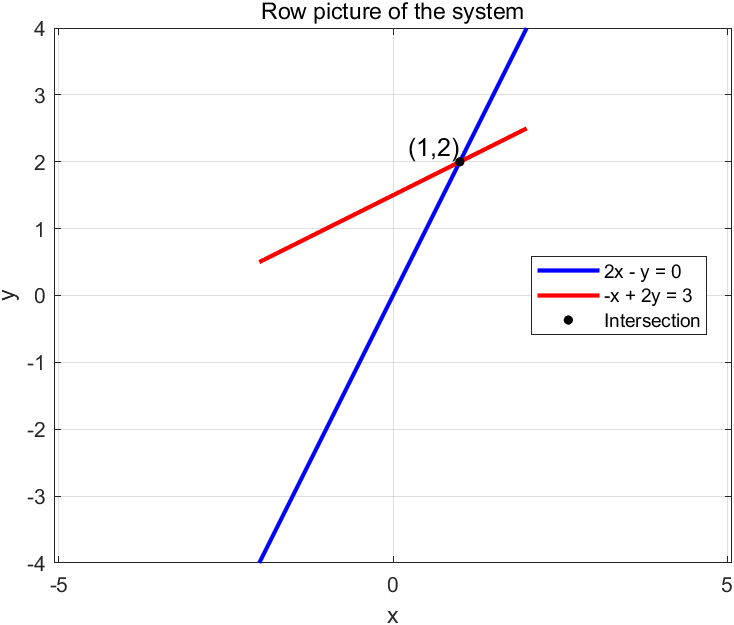
\includegraphics[width=0.8\textwidth]{assets/1.1 Geometric interpretation of
    a system of equations/Row picture.png}
\end{figure}

Now the column picture. When you study linear algebra, you must know that columns are
more important than rows. And you should always think in terms of columns.

eq. (1) can be interpreted as:
\[
  x \begin{bmatrix} 2 \\ -1 \end{bmatrix} +
  y \begin{bmatrix} -1 \\ 2 \end{bmatrix} =
  \begin{bmatrix} 0 \\ 3 \end{bmatrix}
\]

And column picture:
\begin{figure}[H]
    \centering
    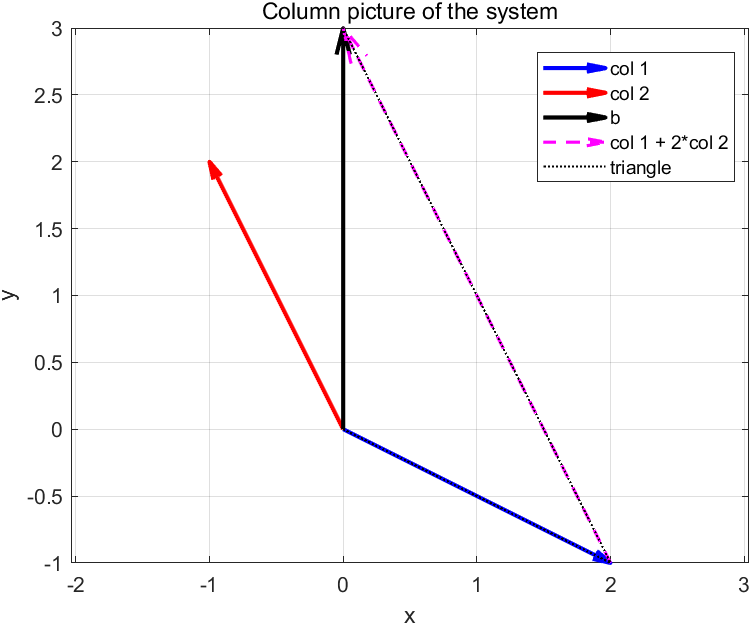
\includegraphics[width=0.8\textwidth]{assets/1.1 Geometric interpretation of
    a system of equations/Column picture.png}
\end{figure}

Now consider a 3-D case:
\begin{equation}
    \begin{aligned}
        a_{11}x + a_{12}y + a_{13}z &= b_1 \\
        a_{21}x + a_{22}y + a_{23}z &= b_2 \\
        a_{31}x + a_{32}y + a_{33}z &= b_3
    \end{aligned}
\end{equation}

If you still think in terms of rows, then you will find that is almost impossible to
visualize it. How can you know where the intersection of three planes is? That's why
we always think in terms of columns.

\subsubsection{\textbf{Solvability of $Ax = b$}}

When you are in middle school, you must heard that some equations system has no solution.
And this is similar to a question in linear algebra: Can $Ax = b$ be solved for any $b$?
For a $n$-D space, this is equal to asking whether the linear combinations of the columns of $A$ can
cover the whole space. If yes, then $Ax = b$ can be solved for any $b$.

For most matrices, the answer is yes. The columns of these matrices are linearly
independent and have ability to cover the whole space. We call these matrices
\textbf{invertible matrices}. And those cannot cover the whole space are called
\textbf{singular matrices}. 

For example, consider a 9-D matrix. If 9 column vectors can cover the whole 9-D space (
which means they are linearly independent), then it's invertible. But if the 9th column
vector is just the same as the 8th, then the combinations of these 9 column vectors can
only cover an 8-D space, which means the matrix is singular.

\subsubsection{\textbf{An example of matrix multiplication}}

Matrix multiplication is a very important operation in linear algebra. It can be
interpreted as a linear combination of the columns of the first matrix. (Note that you
can still think in terms of rows, here we show a column example.)

\[
  \begin{bmatrix} 2 & 5 \\ 1 & 3 \end{bmatrix}
  \begin{bmatrix} 1 \\ 2 \end{bmatrix}
  =
  1 \begin{bmatrix} 2 \\ 1 \end{bmatrix} +
  2 \begin{bmatrix} 5 \\ 3 \end{bmatrix}
  =
  \begin{bmatrix} 12 \\7 \end{bmatrix}
\]

\subsection{\textbf{Matrix elimination}}
\subsubsection{\textbf{Elimination}}

Gauss is a great mathematician. He invented a method to solve linear equations, which is
called \textbf{elimination}. It is a very important method in linear algebra.

Consider a system of equations:
\begin{equation}
    \begin{aligned}
        x + 2y + z &= 2 \\
        3x + 8y + z &= 12 \\
        4y + z &= 2
    \end{aligned}
\end{equation}

We can write it in matrix A:
\[
  \begin{bmatrix}
    1 & 2 & 1 \\
    3 & 8 & 1 \\
    0 & 4 & 1
  \end{bmatrix}
\]

We call the element of $A$ at row $i$ and column $j$ as $A_{ij}$ for convenient. Then
$A_{11}$ is the 1st pivot. Subtract 3 times the 1st row from the 2nd row, and we call
this operation as $(2, 1)$ which means elimnation $A_{21}$. Now we have:
\[
  \begin{bmatrix}
    1 & 2 & 1 \\
    0 & 2 & -2 \\
    0 & 4 & 1
  \end{bmatrix}
\]

Now we should do operation $(3, 1)$. However $A_{31}$ is already 0, so we can skip
this step. The 2nd pivot is $A_{22}$. Next $(3, 2)$, which subtracts 2 times the 2nd row
from the 3rd row:
\[
  \begin{bmatrix}
    1 & 2 & 1 \\
    0 & 2 & -2 \\
    0 & 0 & 5
  \end{bmatrix}
\]

Now we have a upper triangular matrix. This is called $U$.

When will the elimination fail? Actually it happens when the pivots are 0 (Always
remember that pivots \textbf{CANNOT BE 0}) and no row exchange can be done. That is to
say, There are no non-zero elements below the pivots. In this case, the system of
equations has no solution.

After that, we make an argumented matrix $[A\,|\,b]$:
\[
  \left[
  \begin{array}{ccc|c}
    1 & 2 & 1 & 2 \\
    3 & 8 & 1 & 12 \\
    0 & 4 & 1 & 2
  \end{array}
  \right]
  \rightarrow
  \left[
  \begin{array}{ccc|c}
    1 & 2 & 1 & 2 \\
    0 & 2 & -2 & 6 \\
    0 & 0 & 5 & -10
  \end{array}
  \right]
\]

And we call the result $[U|c]$. $c$ is the result of $b$.

\subsubsection{\textbf{Back substitution}}

Now we can solve the system of equations by back substitution. Just solve $Ux = c$.
\begin{equation}
    \begin{aligned}
        5z &= -10 \\
        2y - 2z &= 6 \\
        x + 2y + z &= 2
    \end{aligned}
\end{equation}

This is easy, isn't it?

\subsubsection{\textbf{Elimination matrices}}

Before we go further, we should know that matrix multiplication can be interpreted as
a row operation. For example, a row vector $[1, 2, 7]$ multiples a $3 \times 3$ matrix,
the result is a row vector which is 1 $\times$ row 1 + 2 $\times$ row 2 + 7 $\times$
row 3.

We can get the elimination matrix $E_{ij}$ which is used to eliminate $A_{ij}$. And if
we use the thought above, we can get the elimination matrix:
\[
  E_{21} = \begin{bmatrix}
    1 & 0 & 0 \\
    -3 & 1 & 0 \\
    0 & 0 & 1
  \end{bmatrix}
  \quad
  E_{32} = \begin{bmatrix}
    1 & 0 & 0 \\
    0 & 1 & 0 \\
    0 & -2 & 1
  \end{bmatrix}
\]

The whole elimination process can be written as:
\[
  E_{32} (E_{21} A) = U \quad or \quad (E_{32} E_{21}) A = U
\]

\textbf{P.S.} In matrix multiplication, the associative property holds but the
commutative property does \textbf{not}!

\subsubsection{\textbf{Identity matrix and permutation matrix}}

Identity matrix $I$ is a matrix that has 1s on the diagonal and 0s elsewhere. It is
the multiplicative identity of matrices, which means $AI = A$ and $IA = A$.

Permutation matrix $P$ is a matrix that is used to permute the rows or columns of
another matrix. See the following example:
\[
  \begin{bmatrix}
    0 & 1 \\
    1 & 0
  \end{bmatrix}
  \begin{bmatrix}
    a & b \\
    c & d
  \end{bmatrix}
  =
  \begin{bmatrix}
    c & d \\
    a & b
  \end{bmatrix}
  \quad
  \begin{bmatrix}
    a & b \\
    c & d
  \end{bmatrix}
  \begin{bmatrix}
    0 & 1 \\
    1 & 0
  \end{bmatrix}
  =
  \begin{bmatrix}
    b & a \\
    d & c
  \end{bmatrix}
\]

\subsection{\textbf{Matrix multiplication}}
\subsubsection{\textbf{Definition}}

Matrix multiplication is defined when the number of columns of the first matrix is
equal to the number of rows of the second matrix. For example, a $m \times n$ matrix
$A$ can be multiplied by a $n \times p$ matrix $B$, and the result is a $m \times p$
matrix $C$.

\subsubsection{\textbf{Calculation methods}}

Normally, we have such a equation for individual elements:
\[
  C_{ij} = \sum_{k=1}^{n} A_{ik} B_{kj}
\]

However, this is not the only way to calculate. Don't forget the row and column
interpretation of matrix multiplication. columns of $C$ are linear combinations of
the columns of $A$ with the coefficients from the rows of $B$, or rows of $C$ are linear
combinations of the rows of $B$ with the coefficients from the columns of $A$.

Also, we have the fourth way. $C$ can be represented as columns of $A$ multiplied by
the rows of $B$. Here is an example:
\[
  \begin{bmatrix}
    2 & 7 \\ 3 & 8 \\ 4 & 9
  \end{bmatrix}
  \begin{bmatrix}
    1 & 6 \\ 0 & 0
  \end{bmatrix}
  =
  \begin{bmatrix}
    2 \\ 3 \\ 4
  \end{bmatrix}
  \begin{bmatrix}
    1 & 6
  \end{bmatrix}
  +
  \begin{bmatrix}
    7 \\ 8 \\9
  \end{bmatrix}
  \begin{bmatrix}
    0 & 0
  \end{bmatrix}
  =
  \begin{bmatrix}
    2 & 12 \\ 3 & 18 \\ 4 & 24
  \end{bmatrix}
\]

If the matrices are large, we can cut them into blocks. For example, a $4 \times 4$
matrix can be cut into four $2 \times 2$ blocks. Then we can calculate the blocks
separately and then combine them. This is called \textbf{block matrix multiplication}.
\[
  \begin{bmatrix}
    A_{1} & A_{2} \\
    A_{3} & A_{4}
  \end{bmatrix}
  \begin{bmatrix}
    B_{1} & B_{2} \\
    B_{3} & B_{4}
  \end{bmatrix}
  =
  \begin{bmatrix}
    A_{1}B_{1} + A_{2}B_{3} & A_{1}B_{2} + A_{2}B_{4} \\
    A_{3}B_{1} + A_{4}B_{3} & A_{3}B_{2} + A_{4}B_{4}
  \end{bmatrix}
\]

It is clear that here we use the method 1 to calculate the blocks.

\subsection{\textbf{Inverse}}
\subsubsection{\textbf{Definition}}

We only talk about \textbf{square matrices} in this section. An invertible matrix $A$
has an inverse matrix $A^{-1}$ such that $A^{-1}A = I$ (left inverse) and $AA^{-1} = I$
(right inverse). left inverse and right inverse are the same for square matrices, so we
can say $A^{-1}A = I = AA^{-1}$.

If a matrix is not invertible, then it is called a singular matrix. We have a way to
determine whether a matrix is singular that if there is a $x \neq 0$ makes $Ax = 0$,
then $A$ is singular.

\subsubsection{\textbf{Calculation}}

To calculate the inverse of a matrix is not easy. \textbf{Gauss-Jordan elimination}
gives us a way.

Suppose $A = \begin{bmatrix} 1 & 3 \\ 2 & 7 \end{bmatrix}$, they we can create an
argumented matrix $[A\,|\,I]$:
\[
  \left[
  \begin{array}{cc|cc}
    1 & 3 & 1 & 0 \\
    2 & 7 & 0 & 1
  \end{array}
  \right]
  \rightarrow
  \left[
  \begin{array}{cc|cc}
    1 & 0 & 7 & -3 \\
    0 & 1 & -2 & 1
  \end{array}
  \right]
\]

Now we have $A^{-1} = \begin{bmatrix} 7 & -3 \\ -2 & 1 \end{bmatrix}$ by eliminate the
left part of the argumented matrix to $I$.

But why? This is the smart point of Gauss-Jordan elimination. Calculate $E [A\,|\,I]$
gives $[I\,|\,A^{-1}]$. Well, because $EA = I$ and $A^{-1}A = I$ so $EI = A^{-1}$, clearly.

\subsubsection{\textbf{Some matrices' inverses}}

First one is $AB$, we have:
\[
  A(BB^{-1})A^{-1} = I \quad and \quad B^{-1}(A^{-1}A)B = I \quad \Rightarrow
  \quad (AB)^{-1} = B^{-1}A^{-1}
\]

Second one is $A^{T}$, this is called the transpose of $A$. We will talk about it in
the next chapter detailly. Here we just have to know that transpose is to swap the rows
and columns of a matrix. And we have:
\[
  AA^{-1} = I \quad \Rightarrow \quad (A^{-1})^{T} A^{T} = I \quad \Rightarrow \quad
  (A^{T})^{-1} = (A^{-1})^{T}
\]

That is to say, inverse and transpose can exchange their order for a matrix.

\subsection{\textbf{LU factorization}}
\subsubsection{$A = LU$}

Through eliminate, we have get $EA = U$, where $E$ is the elimination matrix and $U$ is
the upper triangular matrix. And we can change it to $A = LU$, where $L$ is the lower
triangular matrix. This is called \textbf{LU factorization}. Also, we assume that $A$
dosen't need row exchanges in this subsection.

Suppose elimination of a $3 \times 3$ matrix $A$:
\[
  E_{32}E_{31}E_{21} A = U \quad \Rightarrow \quad A = E_{21}^{-1}E_{31}^{-1}E_{32}^{-1}U
\]

So we have:
\[
  L = E_{21}^{-1}E_{31}^{-1}E_{32}^{-1}
\]

You may ask, is there a necessity to do this? Yes, here is an example to tell the reason.
\[
  E = \begin{bmatrix}
    1 & 0 & 0 \\
    0 & 1 & 0 \\
    0 & -5 & 1
  \end{bmatrix}
  \begin{bmatrix}
    1 & 0 & 0 \\
    -2 & 1 & 0 \\
    0 & 0 & 1
  \end{bmatrix}
  =
  \begin{bmatrix}
    1 & 0 & 0 \\
    -2 & 1 & 0 \\
    10 & -5 & 1
  \end{bmatrix}
\]

\[
  L = \begin{bmatrix}
    1 & 0 & 0 \\
    2 & 1 & 0 \\
    0 & 0 & 1
  \end{bmatrix}
  \begin{bmatrix}
    1 & 0 & 0 \\
    0 & 1 & 0 \\
    0 & 5 & 1
  \end{bmatrix}
  =
  \begin{bmatrix}
    1 & 0 & 0 \\
    2 & 1 & 0 \\
    0 & 5 & 1
  \end{bmatrix}
\]

What can you see? $2$ and $5$ are the multipliers of the elimination. And they don't
conflict with each other in $L$. So writing $L$ really don't need calculations. What
you need to do is just to write down the multipliers of the elimination. And this is
exactly the reason why $L$ is better.

\subsubsection{$PA = LU$ \textbf{, permutation matrix and transpose}}

Not all matrices can be eliminated without row exchanges. So we have to use permutation
matrices $P$ to do row exchanges. Then we have $PA = LU$. This is called \textbf{LU
factorization with pivoting}.

Here we will talk more about $P$. There is a important property of $P$:
\[
  P^{-1} = P^{T} \quad or \quad P^{2} = P^{T}P = I
\]

Also the transpose:
\[
  (A_{ij})^{T} = A_{ji}
\]

Till now, we can introduce a property of matrix called \textbf{symmetric}. A matrix $A$
is symmetric if $A^{T} = A$. A rectangle matrix $R$ follows that $R^{T}R$ is symmetric.
Here's the proof:
\[
  (R^{T}R)^{T} = R^{T}R^{TT} = R^{T}R
\]

Remember, inverse and transpose exchange matrix order.

\newpage
\thispagestyle{empty}
\begin{center}
    \vspace*{96pt}
    \fontsize{60}{60}\customfont{2}\par
    \fontsize{26}{31.2}\section{\textbf{Vector spaces}}\par % 标题
    \vspace{25pt}
    \begin{center}
      \fontsize{18}{21.6}\customfont\textit{The important thing is not to stop
    questioning. Curiosity has its own reason for existing.}
    \end{center}
    \begin{flushright}
      \fontsize{18}{21.6}\customfont\textit{--- Albert Einstein}
    \end{flushright}
    \vfill
\end{center}

\fontsize{12}{14}
\newpage
\subsection{\textbf{Vector space and subspace}}

A vector space is a set of vectors that can be added together and multiplied by scalars
(scalars are real numbers). A vector space must satisfy many properties. But we don't
need to know all of them. Here we just need to know that a vector space is closed under
addition and scalar multiplication. That is to say, if $u$ and $v$ are in a vector space
$V$, then $u + v$ and $cu$ (where $c$ is a scalar) are also in $V$. Further, it equals
to that $cu + dv$ (where $c$ and $d$ are scalars) is also in $V$.

We define $R^{n}$ as the set of all $n$-dimensional vectors. It is a vector space.

If we draw a 2-D coordinate system, and point the 1st quadrant, is this a vector space?
Absolutely not. Because it is not closed under addition. For example, if we multiple a
vector by $c = -1$, then the vector will be in the 3rd quadrant, which tells us that
the 1st quadrant is not closed so not a vector space.

Subspace is a subset of a vector space that is also a vector space. Let's take $R^{2}$
as an example. There are 3 subspaces of $R^{2}$: the zero vector ($Z$), a line through
the origin ($L$) and the whole $R^{2}$ itself. Notice that not all lines are subspaces
except the lines through the origin point, because only this matches definition when
$c = 0$.

What about $R^{3}$? There are 4 subspaces: the zero vector, a plane through the origin,
a line through the origin and the whole $R^{3}$ itself. Again, not all planes are
subspaces except the planes through the origin.

Let's be next, consider two subspaces $P$ and $L$ of $R^{3}$. Is $P \cap L$ a subspace?
No. Because it is not closed under addition. 2 vectors, one in $P$ and the other in $L$,
their sum may not be in $P \cap L$. What about $P \cup L$? Yes. And this forms a smaller
subspace. Normally, subspace intersection is a subspace, but union is not.

\subsection{\textbf{Column space and null space}}

Column space $C(A)$ is the set of all linear combinations of the columns of a matrix
$A$. It is a subspace of $R^{m}$, where $m$ is the number of rows of $A$.

For example, consider a matrix:
\[
  A = \begin{bmatrix}
    1 & 1 & 2 \\
    2 & 1 & 3 \\
    3 & 1 & 4 \\
    4 & 1 & 5 \\
  \end{bmatrix}
\]

The column space of $A$ is the set of all linear combinations of the columns of $A$:
\[
  C(A) = \{ c_1 \begin{bmatrix} 1 \\ 2 \\ 3 \\ 4 \end{bmatrix} +
           c_2 \begin{bmatrix} 1 \\ 1 \\ 1 \\ 1 \end{bmatrix} +
           c_3 \begin{bmatrix} 2 \\ 3 \\ 4 \\ 5 \end{bmatrix}
           \,|\, c_1, c_2, c_3 \in R \}
\]

And here we can see that $C(A)$ is a 2-D space in $R^{4}$. So there is not every $b$
can make $Ax = b$ solvable. In fact, only when $b$ is in $C(A)$, then $Ax = b$ can be
solved.

Null space $N(A)$ is the set of all solutions to equation $Ax = 0$. It is important
that $N(A)$ is a subspace of $R^{n}$ (Not $m$!), where $n$ is the number of columns of
$A$.

Most of the time, $N(A)$ is solved by elimination. And when the matrix is invertible,
then $N(A) = \{0\}$. It's said that only singular matrices have non-trivial null
spaces.

\subsection{\textbf{Solution of $Ax = 0$ and} \textit{rref()}}
\subsubsection{\textbf{Solution of $Ax = 0$}}
Consider a matrix:
\[
  A = \begin{bmatrix}
    1 & 2 & 2 & 2 \\
    2 & 4 & 6 & 8 \\
    3 & 6 & 8 & 10
  \end{bmatrix}
\]

We can eliminate it to:
\[
  U = \begin{bmatrix}
    1 & 2 & 2 & 2 \\
    0 & 0 & 2 & 4 \\
    0 & 0 & 0 & 0
  \end{bmatrix}
\]

And $U$ is called row echelon form of $A$.

\vspace{0.5em}
\textbf{P.S.} Elimination does not change $N(A)$.
\newpage
Here we need to tell some definitions.
\begin{itemize}
  \item \textbf{Rank}: The number of non-zero rows in echelon form of a matrix.
  \item \textbf{Pivot column}: The column that contains a pivot.
  \item \textbf{Free column}: The column that does not contain a pivot.
\end{itemize}

Pivot columns and free columns are important. The variables corresponding to free
columns can be arbitrary, while the variables corresponding to pivot columns are
determined by the free variables. In this example, $x_2$ and $x_4$ are free variables,
while $x_1$ and $x_3$ are pivot variables. If we let $x_2 = 1$ and $x_4 = 0$, then
$x_1 = -2$ and $x_3 = 0$. So one solution is:
\[
  x = \begin{bmatrix}
    -2 \\ 1 \\ 0 \\ 0
  \end{bmatrix}
\]

And we can also get another solution:
\[
  x = \begin{bmatrix}
    2 \\ 0 \\ -2 \\ 1
  \end{bmatrix}
\]

These two solutions are called \textbf{special solutions}. The special solutions
form $N(A)$. And the number of special solutions is equal to the number of free
columns. Here we have 2 free columns, so $N(A)$ is a 2-D space in $R^{4}$.
\[
  N(A) = \left\{ c_1 \begin{bmatrix} -2 \\ 1 \\ 0 \\ 0 \end{bmatrix} +
               c_2 \begin{bmatrix} 2 \\ 0 \\ -2 \\ 1 \end{bmatrix}
               \,|\, c_1, c_2 \in R \right\}
\]

So the conclusion is that for a $m \times n$ matrix of rank $r$, the number of free
columns is $n - r$ which means that $N(A)$ is a $(n - r)$-D space in $R^{n}$.

\subsubsection{\textit{rref()}}

Now let's talk about a matrix $R$ which is called \textbf{reduced row echelon form}
of $A$. It is got by further eliminating $U$ to make the pivots be 1 and the other
elements in the pivot columns be 0 as much as possible. Here is the result of the
example above:
\[
  R = \begin{bmatrix}
    1 & 2 & 0 & 2 \\
    0 & 0 & 1 & 2 \\
    0 & 0 & 0 & 0
  \end{bmatrix}
\]

This matrix can be generated by the \textit{rref()} function in MATLAB.

If we sort the pivot columns of together and free columns together, then we can get
\[
  R = \begin{bmatrix}
    1 & 0 & 2 & 2 \\
    0 & 1 & 0 & 2 \\
    0 & 0 & 0 & 0
  \end{bmatrix}
\]

Here you may ask why we spend time introducing $R$, you should know everything in this
brief tutorial must be valuable xD

Pivot columns creates $I$, and we call the other part $F$:
\[
  R = \begin{bmatrix}
    I & F \\
    0 & 0
  \end{bmatrix}
\]

Let's create a nullspace matrix $N$ that $RN = 0$, then we have:
\[
  N = \begin{bmatrix}
    -F \\ I
  \end{bmatrix}
\]

Do you see it? This is exactly the special solutions we talked about before.
So we can use \textit{rref()} to solve $N(A)$ quite easily.

\subsection{\textbf{Complete solution of $Ax = b$}}

Just like $Ax = 0$, $Ax = b$ is solvable only when $b$ is in $C(A)$.

If you have learned Teacher Ji's (or Teacher Jiang's) Circuit Analysis course, then
you must know that the complete solution of a differential equation is the sum of a
particular solution and the general solution (Actually this is already talked in
Higher Mathematics).

This is also true for $Ax = b$. The complete solution is the sum of a particular
solution $x_p$ and the general solution $x_n$.

When solving $x_p$, make free variables 0 to avoid the general solution part. And
use \textit{rref()} to solve $x_n$.

As the example in the last section, we can get the result:
\[
  x_c = x_p + x_n =
  \begin{bmatrix}
    -2 \\ 0 \\ 3/2 \\ 0
  \end{bmatrix} +
  c_1 \begin{bmatrix} -2 \\ 1 \\ 0 \\ 0 \end{bmatrix} +
  c_2 \begin{bmatrix} 2 \\ 0 \\ -2 \\ 1 \end{bmatrix}
  \quad c_1, c_2 \in R
\]

Above is the normal case. Now we consider 4 special cases.

First, when $r = n < m$. This is the case of full column rank. Here $N(A) = \{0\}$, so
the complete solution is just the particular solution. And $Ax = b$ has either 0 or 1
solution. And only when $b$ is in $C(A)$, then $Ax = b$ has 1 solution.

Second, when $r = m < n$. This is the case of full row rank. Here $C(A) = R^{m}$, so
$Ax = b$ is solvable for any $b$. And $Ax = b$ has either 1 or infinite solutions.
And only when $N(A) = \{0\}$, then $Ax = b$ has 1 solution.

Third, when $r = m = n$. This is the case of full rank. Here $A$ is invertible, so
$Ax = b$ has exactly 1 solution for any $b$. And $N(A) = \{0\}$.

Last, when $r < m$ and $r < n$. This is the case of low rank. Here $Ax = b$ has either 0 or
infinite solutions. When $b$ is in $C(A)$, then $Ax = b$ has infinite solutions.

\subsection{\textbf{Linear independence, basis and dimension}}
\subsubsection{\textbf{Linear independence}}

A set of vectors is linearly independent if the only solution to the equation
\[
  c_1 v_1 + c_2 v_2 + \cdots + c_n v_n = 0
\]

is $c_1 = c_2 = \cdots = c_n = 0$. Otherwise, the set is linearly dependent.

If all column vectors of a matrix are linearly independent, then the nullspace of
the matrix is $\{0\}$. And the matrix is of full column rank.

\subsubsection{\textbf{Basis and dimension}}

Before basis, we need to introduce span. The span of a set of vectors is the set of all
linear combinations of those vectors. For example, the span of two linearly independent
vectors in $R^{2}$ is the whole 2-D space.

Basis of a vector space is a set of linearly independent vectors that span the space.

For example, the standard basis of $R^{3}$ is:
\[
  e_1 = \begin{bmatrix} 1 \\ 0 \\ 0 \end{bmatrix}, \quad
  e_2 = \begin{bmatrix} 0 \\ 1 \\ 0 \end{bmatrix}, \quad
  e_3 = \begin{bmatrix} 0 \\ 0 \\ 1 \end{bmatrix}
\]

There are 2 important properties about basis. First, every set of bases of a vector
space is invertible (because they are linearly independent). Second, every set of bases of a vector
space has the same number of vectors, this number is called the \textbf{dimension} of
the vector space. For a 2-D matrix $A$, we say that $\dim(A) = 2$.

Now we come to the most beautiful part. There is a equation:
\[
  \text{rank}(A) = \dim(C(A)) \quad \& \quad \text{rank}(A) + \dim(N(A)) = n
\]

It's obvious that $\dim(N(A)) = n - r$. But why $\dim(C(A)) = r$? Because the pivot
columns of $A$ form a basis of $C(A)$. This is easy to prove. First, pivot columns
are linearly independent. Second, any column of $A$ can be expressed as a linear
combination of the pivot columns. So the pivot columns span $C(A)$. So they form a
basis of $C(A)$.

\subsection{\textbf{Four fundamental subspaces}}

There are 4 fundamental subspaces of a matrix $A$:
\begin{itemize}
  \item Column space $C(A)$, a subspace of $R^{m}$
  \item Null space $N(A)$, a subspace of $R^{n}$
  \item Row space $C(A^{T})$, a subspace of $R^{n}$
  \item Left null space $N(A^{T})$, a subspace of $R^{m}$
\end{itemize}

And we have:

\begin{align*}
  \dim(C(A)) &= \dim(C(A^{T})) = r \\
  \dim(N(A)) &= n - r  \\
  \dim(N(A^{T})) &= m - r
\end{align*}

In section 2.2, we have talked about $C(A)$ and $N(A)$. So this section we will focus
on $C(A^{T})$ and $N(A^{T})$.

$C(A^{T})$ is the row space of $A$. The basis of $C(A^{T})$ are the non-zero rows of
$R$. And the rank of it is also $r$ because the number of non-zero rows is also the
same as the number of pivots.

$N(A^{T})$ is the left null space of $A$. It is the set of all solutions to equation
$A^{T}y = 0$. The basis of $N(A^{T})$ can be found by solving $R^{T}y = 0$. Here's
an example:
\[
  A = \begin{bmatrix}
    1 & 2 & 3 & 1 \\
    1 & 1 & 2 & 1 \\
    1 & 2 & 3 & 1
  \end{bmatrix}
\]

Remember LU factorization? Here we have $EA = R$:
\[
  E = \begin{bmatrix}
    -1 & 2 & 0 \\
    1 & -1 & 0 \\
    -1 & 0 & 1 \\
  \end{bmatrix}
  \quad
  R = \begin{bmatrix}
    1 & 0 & 1 & 1 \\
    0 & 1 & 1 & 0 \\
    0 & 0 & 0 & 0
  \end{bmatrix}
\]

See $EA = R$ in row view, $m - r$ rows vector in the bottom of $E$ makes $EA = 0$.
In this example, $m - r = 1$, so the last row of $E$ is a basis of $N(A^{T})$.

\subsection{\textbf{Graph and network}}
\subsubsection{\textbf{Graph}}

Here is an example of a graph:
\begin{figure}[H]
  \centering
  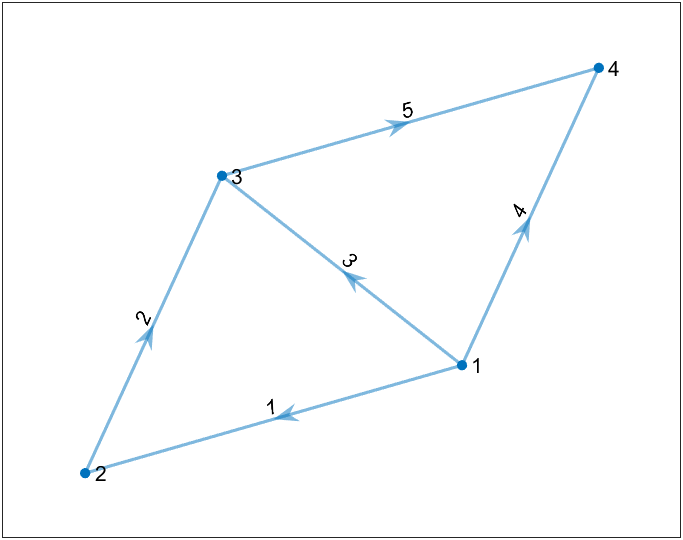
\includegraphics[width=0.56\textwidth]{assets/2.7 Graph and network/Graph.png}
  \caption{A graph with 4 nodes and 5 edges}
\end{figure}

This can represent many things, such as a road map, a social network and so on.
And we assume that it's a circuit. The whole graph can be represented by a\textbf{
incidence matrix} $A$, where rows represent nodes and columns represent edges, and
1 means current flows into the node, -1 means current flows out of the node:
\[
  A = \begin{bmatrix}
    -1 & 1 & 0 & 0 \\
    0 & -1 & 1 & 0 \\
    -1 & 0 & 1 & 0 \\
    -1 & 0 & 0 & 1 \\
    0 & 0 & -1 & 1
  \end{bmatrix}
\]

And we call a closed figure in a graph as a \textbf{loop}. Here we have 2 loops, let's
take 1->2->3->1 as an example. If we walk along the loop, then we can get a zero sum.
So do Kirchhoff's Law. And in this tutorial we don't talk much about this. We pay more
attention to the independence of loops. Obviously, edge 1, 2 and 3 are linear dependent.

A deeper question is that are these columns of $A$ linear independent?

It can't be seen directly. Let's think about $Ax = 0$. Don't forget the physical meaning of
a circuit. $x$ means potentials at nodes. So $Ax = 0$ means that the potential
difference at each edge is 0. This is true when all nodes have the same potential (except for
all zero case). So $N(A) = \{c[1, 1, 1, 1]^T \,|\, c \in R\}$ which means that the columns of
$A$ are linear dependent.

Now we have the conclusion that for arbitrary 3 nodes, the columns of $A$ are linear
independent. But when we add a 4th node, the columns of $A$ become linear dependent.
This means that rank of $A$ is 3. In fact, we often ground the 4th node to make $A$ be of
full column rank.

What about $N(A^{T})$? Well $y$ in $A^{T}y = 0$ symbolizes the currents in edges. $x$ and
$y$ obey Ohm's Law. To solve $A^{T}y = 0$, we can use Kirchhoff's Current Law. I won't
go into details here.

If edge 3 and 4 are deleted, then the graph becomes a \textbf{tree}. A tree is a graph
with no loops.

\subsubsection{\textbf{Inference}}

We already know that $N(A^{T}) = m - r$ and $r = n - 1$ in a connected graph. So we have:
\[
  \# loops + \# nodes - \# edges = 1
\]

This is called \textbf{Euler's formula}. It explains the structure of a graph well. When
facing a complex graph, we can use this formula to check whether our analysis is right.

A very important example is the \textbf{branch current method}. For a $b$ edges circuit with
$n$ nodes, KCL gives $n - 1$ independent equations, and resistances give $b$ independent
equations, and KVL gives $b - (n - 1)$ independent equations just because of Euler's formula.

Also, from the derivation above we can conclude matrix form of Kirchhoff's Laws.

We call current potential difference as $e$ then $Ax = e$, resistance matrix as $C$ then
$y = Ce$ and external power supply influence as $f$. So we have:
\[
  A^{T}y = A^{T}Ce = A^{T}CAx = f
\]

\newpage
\thispagestyle{empty}
\begin{center}
    \vspace*{96pt}
    \fontsize{60}{60}\customfont{3}\par
    \fontsize{26}{31.2}\section{\textbf{Orthogonality}}\par % 标题
    \vspace{25pt}
    \begin{center}
      \fontsize{18}{21.6}\customfont\textit{Logic is the foundation of the certainty of all
      the knowledge we acquire.}
    \end{center}
    \begin{flushright}
      \fontsize{18}{21.6}\customfont\textit{--- Leonhard Euler}
    \end{flushright}
    \vfill
\end{center}

\newpage
\subsection{\textbf{Orthogonal vector and orthogonal subspace}}
\subsubsection{\textbf{Definition}}

Orthogonality is common in mathematics. Two vectors are orthogonal if their dot product
is 0. That is:
\[
  u \cdot v = 0 \quad or \quad u^{T}v = 0
\]

Two subspaces are orthogonal if every vector in one subspace is orthogonal to every
vector in the other subspace. However, there are some counterintuitive situations.
For example, consider the $x-y$ plane and the $y-z$ plane in $R^{3}$. They are not
orthogonal because the line $c[0, 1, 0]^T$ is in both planes.


Actually we can say that two subspaces are orthogonal only when their intersection is
$\{0\}$. Otherwise, they must be not orthogonal. 

\subsubsection{\textbf{Orthogonal complement}}

Row space $C(A^{T})$ and null space $N(A)$ are orthogonal. Left null space $N(A^{T})$
and column space $C(A)$ are orthogonal.

Here we take $C(A^{T})$ and $N(A)$ as an example to prove. Suppose $x \in N(A)$, then
we know that $Ax = 0$. See this formula as a matrix multiplication, every rows of $A$
is orthogonal to $x$. And the linear combinations of the rows of $A$ are also orthogonal to
$x$. So every vector in $C(A^{T})$ is orthogonal to every vector in $N(A)$. This confirms
th defination of orthogonal subspaces.

But it is not end here. We know that $\dim(C(A^{T})) + \dim(N(A)) = n$. That is to say,
$C(A^{T})$ and $N(A)$ together span $R^{n}$. So $N(A)$ contains all vectors that are
orthogonal to $C(A^{T})$. This is called \textbf{orthogonal complement}. And this is also
true for $N(A^{T})$ and $C(A)$.

\subsection{\textbf{Orthogonal projection}}
\subsubsection{\textbf{Derivation}}

Projection of a vector $b$ onto a subspace $S$ is to find a vector $p$ in $S$ that is
closest to $b$. The error vector $e = b - p$ is orthogonal to $S$. This is called
\textbf{orthogonal projection}.
\begin{figure}[H]
  \centering
  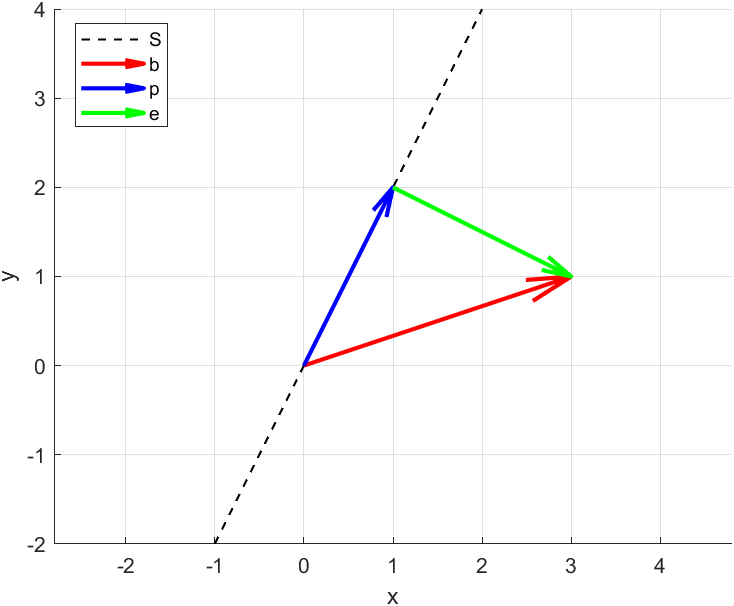
\includegraphics[width=0.6\textwidth]{assets/3.2 Orthogonal projection/Orthogonal projection.png}
  \caption{Orthogonal projection}
\end{figure}

We know $p$ is on $S$, assume there is a vector $a$ that spans $S$, then $p = xa$. Then we
have:
\[
  a^{T}(b - xa) = 0 \quad \Rightarrow \quad x = \frac{a^{T}b}{a^{T}a}
\]

If we define a projection matrix $P$ that $p = Pb$, then we have:
\[
  p = \frac{a a^{T}}{a^{T}a} b \quad \Rightarrow \quad P = \frac{a a^{T}}{a^{T}a}
\]

Obviously, $P$ is a symmetric matrix which means $P^{T} = P$, also $rank(P) = 1$ because
$P$ is the product of two vectors. And $P^{2} = P$ because projecting twice is the same as
projecting once.

May you ask why we need projection? The core is to solve $Ax = b$ when no solution exists.
What we can do is to project $b$ onto $C(A)$ to get $p$, then solve $A \hat{x} = p$. This
is called \textbf{least squares solution}.

For a higher dimensional subspace $S$, the method is similar. We also have $A^{T}(b -
A\hat{x}) = 0$, then:
\[
  \hat{x} = (A^{T}A)^{-1}A^{T}b \quad and \quad P = A(A^{T}A)^{-1}A^{T}
\]

And the properties of $P$ are the same as before. By the way, this is the kernel of
\textbf{least squares method}.

\subsubsection{\textbf{An important proof of $A^{T}A$}}

There is a important property of $A^{T}A$ that if $A$ has linear independent columns,
then $A^{T}A$ is invertible. Here is the proof.

Suppose $A^{T}Ax = 0$. We must prove that $x = 0$. We can play a trick:
\[
  x^{T}A^{T}Ax = (Ax)^{T}(Ax) = ||Ax||^{2} = 0 \quad \Rightarrow \quad Ax = 0
\]

Because $A$ has linear independent columns, then $x = 0$. So the proof is complete.

\subsection{\textbf{Orthogonal basis and orthogonal matrix}}
\subsubsection{\textbf{Orthogonal basis}}

No one wants to see lots of square roots in calculations. So orthogonal basis is defined
as a set of \textbf{orthonormal vectors} that span a space. Orthonormal means that the
vectors are orthogonal and of unit length, here is the formula:
\[
  q_i^{T}q_j = \begin{cases}
    1 & i = j \\
    0 & i \neq j
  \end{cases}
\]

And orthogonal basis contains $q_1, q_2, \ldots, q_n$. By the way, it is column basis
normally.

\subsubsection{\textbf{Orthogonal matrix}}

Orthogonal matrix $Q$ is a \textbf{square} (not a must but usually) matrix whose columns
form an orthonormal basis. And we have:
\[
  Q^{T}Q = I \quad or \quad Q^{-1} = Q^{T}
\]

Here is a famous example of orthogonal matrix called \textbf{Adhmar matrix} $H$:
\[
  H_4 = \frac12 \begin{bmatrix}
    1 & 1 & 1 & 1 \\
    1 & -1 & 1 & -1 \\
    1 & 1 & -1 & -1 \\
    1 & -1 & -1 & 1
  \end{bmatrix}
\]

$\frac12$ is used to make the columns be of unit length. And $H$ is widely used in
signal processing.

If we project $Q$ onto its column space, then we get $Q$'s $P$:
\[
  P = Q(Q^{T}Q)^{-1}Q^{T} = QQ^{T}
\]

When $Q$ is a square matrix, then $P = I$.

Now we can rewrite the least squares formula:
\[
  Q^{T}Q\hat{x} = Q^{T}b \quad \Rightarrow \quad \hat{x} = Q^{T}b
\]

That means $\hat{x_i} = $$q_i^{T}b$.

\subsection{\textbf{QR factorization}}
\subsubsection{\textbf{Gram-Schmidt process}}

Gram-Schmidt process is a method to convert a set of basis to an orthogonal basis. Suppose
we have three vectors $a, b, c$, then we can convert them to orthogonal vectors $q_1, q_2,
q_3$.

First, we should change $a, b, c$ to orthogonal. This step is the same as 3.2.1. If we
call the result $A, B, C$, then we have:
\begin{align*}
  A &= a \\
  B &= b - \frac{A^{T}b}{A^{T}A}A \\
  C &= c - \frac{A^{T}c}{A^{T}A}A - \frac{B^{T}c}{B^{T}B}B
\end{align*}

Take a look at $C$, we already know $B$ is orthogonal to $A$, so we just need to do the
following steps twice to get $C$.

Finally, make $A, B, C$ be of unit length to get $q_1, q_2, q_3$:
\[
  q_1 = \frac{A}{||A||}, \quad q_2 = \frac{B}{||B||}, \quad q_3 = \frac{C}{||C||}
\]

\subsubsection{\textbf{QR factorization}}

QR factorization is another important method to factor a matrix $A$, which decompose
$A$ into the product of an orthogonal matrix $Q$ and an upper triangular matrix $R$:
\[
A = QR
\]

$R$ contains the coefficients from Gram-Schmidt process. Here's a example of $2 \times 2$
matrix.
\[
  Q = \begin{bmatrix} q_1 & q_2 \end{bmatrix} \quad
  R = \begin{bmatrix}
    a_1^{T}q_1 & a_2^{T}q_2 \\
    a_1^{T}q_2 & a_2^{T}q_1
  \end{bmatrix}
\]

\newpage
\thispagestyle{empty}
\begin{center}
    \vspace*{96pt}
    \fontsize{60}{60}\customfont{4}\par
    \fontsize{26}{31.2}\section{\textbf{Determinants}}\par % 标题
    \vspace{25pt}
    \begin{center}
      \fontsize{18}{21.6}\customfont\textit{It is not knowledge, but the act of learning,
      not the possession of but the act of getting there, which grants the greatest
      enjoyment.}
    \end{center}
    \begin{flushright}
      \fontsize{18}{21.6}\customfont\textit{--- Friedrich Gauss}
    \end{flushright}
    \vfill
\end{center}

\newpage
\subsection{\textbf{Determinants and its properties}}
\subsubsection{\textbf{Determinants with properties 1, 2 and 3}}

This is the first chapter of TJU's Linear Algebra book. The difference is striking.

To start with, we need to know what is a determinant. A determinant is a special number
that can be calculated from a \textbf{square matrix}. It is denoted as $det(A)$ or
$|A|$. It is difficult to understand a definition given out of air, so let's start from
determinants's properties 1, 2:
\begin{enumerate}[(1)]
  \item $\det I = 1$
  \item If we exchange two rows, then the determinant changes its sign.
\end{enumerate}

Now the property 3:
\begin{align*}
  \begin{vmatrix}
    ta & tb \\
    c & d
  \end{vmatrix} &=
  t \begin{vmatrix}
    a & b \\
    c & d
  \end{vmatrix} \tag{3a}\\
  \begin{vmatrix}
    a + a' & b + b' \\
    c & d
  \end{vmatrix} &=
  \begin{vmatrix}
    a & b \\
    c & d
  \end{vmatrix}
  +
  \begin{vmatrix}
    a' & b' \\
    c & d
  \end{vmatrix} \tag{3b}
\end{align*}

Here is a important thing to notice of property 3b. This symbolizes that every row
is linear but not the matrix. So it is \textbf{WRONG} to say that $\det(A + B) =
\det A + \det B$.

\subsubsection{\textbf{Properties 4 to 10}}

\begin{enumerate}[start=4,label=(\arabic*)]
  \item If a matrix has same rows, then its determinant is 0.
  \item Subtract a multiple of one row from another row does not change the determinant.
  \item If a matrix has a row of zeros, then its determinant is 0.
  \item For an upper triangular matrix, its determinant is the product of its diagonal
entries.
  \item $\det A = 0$ when $A$ is singular.
  \item $\det AB = (\det A)(\det B)$
  \item $\det A^{T} = \det A$
\end{enumerate}

You may complain that there are too many properties. But they are all simple and useful.
I will explain some more upon them.

Properties 4 and 6 are the same because property 5.

It's easy to prove property 5. See this:
\[
  \begin{vmatrix}
    a & b \\
    c-la & d-lb
  \end{vmatrix} =
  \begin{vmatrix}
    a & b \\
    c & d
  \end{vmatrix} -
  l \begin{vmatrix}
    a & b \\
    a & b
  \end{vmatrix} =
  \begin{vmatrix}
    a & b \\
    c & d
  \end{vmatrix}
\]

For property 7, an upper triangular matrix $U$ can be eliminated to $R$, which is all
zeros except for the pivots. And $\det U = \det R$ because of property 5. Then use
property 3a to get $\det R = $ product of pivots.

Property 8 is the same as property 6 by elimination.

Property 9 tells us 3 things.
\begin{align*}
  \det A^{-1} &= 1/\det A \\
  \det A^2 &= (\det A)^2 \\
  \det mA &= m^n \det A
\end{align*}

\subsection{\textbf{Formula of determinants and Cofactor}}
\subsubsection{\textbf{Formula of determinants}}

First we calculate the determinant of a $2 \times 2$ matrix:
\[
  \begin{vmatrix}
    a & b \\
    c & d
  \end{vmatrix} =
  \begin{vmatrix}
    a & 0 \\
    0 & d-bc/a
  \end{vmatrix} =
  ad - bc
\]

What about a $3 \times 3$ matrix? Elimination will be a not-so-good choice, so we
think about a new way, which uses property 3b:
\[
  \begin{vmatrix}
    a_{11} & a_{12} & a_{13} \\
    a_{21} & a_{22} & a_{23} \\
    a_{31} & a_{32} & a_{33}
  \end{vmatrix} =
  \begin{vmatrix}
    a_{11} & 0 & 0 \\
    0 & a_{22} & 0 \\
    0 & 0 & a_{33}
  \end{vmatrix} +
  \begin{vmatrix}
    a_{11} & 0 & 0 \\
    0 & 0 & a_{23} \\
    0 & a_{32} & 0
  \end{vmatrix} +
  \cdots
\]

Actually there are 6 terms in total. And we should pay attention to the signs. The
result is:
\[
  \det A = a_{11}a_{22}a_{33}-a_{11}a_{23}a_{32}-
           a_{12}a_{21}a_{33}+a_{12}a_{23}a_{31}+
           a_{13}a_{21}a_{32}-a_{13}a_{22}a_{31}
\]

And we can summarize it to a simpler form:
\[
  \det A = \sum_{n!}\pm a_{1i}a_{2j}a_{3k} \cdots a_{nm}
  \quad (i, j, k, \ldots, m \text{ are permutations of } 1, 2, 3, \ldots, n)
\]

\subsubsection{\textbf{Cofactor}}

Cofactor is a useful tool to calculate determinants. The cofactor $C_{ij}$ is defined as:
\[
  C_{ij} = (-1)^{i+j}M_{ij}
\]

$M_{ij}$ is the \textbf{minor} of $a_{ij}$, which is the determinant of the matrix that
removes the $i$-th row and $j$-th column of $A$.

And the determinant of $A$ can be calculated by:
\[
  \det A = \sum_{j=1}^{n} a_{ij}C_{ij} = \sum_{i=1}^{n} a_{ij}C_{ij}
\]

This seems complicated, so let's see an example:
\begin{align*}
  \begin{vmatrix}
    a_{11} & a_{12} & a_{13} \\
    a_{21} & a_{22} & a_{23} \\
    a_{31} & a_{32} & a_{33}
  \end{vmatrix} &=
  a_{11}C_{11} + a_{12}C_{12} + a_{13}C_{13} \\
  C_{11} &= \begin{vmatrix}
    a_{22} & a_{23} \\
    a_{32} & a_{33}
  \end{vmatrix} \\
  C_{12} &= - \begin{vmatrix}
    a_{21} & a_{23} \\
    a_{31} & a_{33}
  \end{vmatrix} \\
  C_{13} &= \begin{vmatrix}
    a_{21} & a_{22} \\
    a_{31} & a_{32}
  \end{vmatrix}
\end{align*}

In fact cofactors decrease a matrix's order by 1. So we can use cofactors to calculate
low order determinants more efficiently. But when facing a much high order matrix, this
method's complexity is too high. So we have to use elimination.

\subsection{\textbf{Cramer's rule}}
\subsubsection{\textbf{Formula of $A^{-1}$}}

We assume a cofactor matrix $C$ which contains all cofactors of $A$. And we have:
\[
  A^{-1} = \frac{1}{\det A} C^{T}
\]

To prove this, we need to prove that $AC^{T} = (\det A)I$. See $AC^{T}$ as a matrix
multiplication, then the element at the $i$-th row and $j$-th column is:
\[
  (AC^{T})_{ij} = \sum_{k=1}^{n} a_{ik}C_{jk}
\]

When $i = j$, this is exactly the formula of $\det A$. When $i \neq j$, this is 0. That's
over.

This is quite hard to understand, let's explain it in detail. When $i \neq j$, we have:
\[
  (AC^{T})_{ij} = \sum_{k=1}^{n} a_{ik}C_{jk} =
  \det B
\]

$B$ is the matrix that replaces the $j$-th row of $A$ with its $i$-th row. ($a_{ik} \,
\text{becomes} \, b_{jk}$). Because $B$ has two same rows, then $\det B = 0$.

\subsubsection{\textbf{Cramer's rule}}

According to $Ax = b$, and the formula of $A^{-1}$, we have:
\[
  x = A^{-1}b = \frac{1}{\det A} C^{T}b
\]

$C^{T}b$ can be seen as a determinant of a new matrix $B$, and we can get:
\[
  x_i = \frac{\det B_i}{\det A}
\]

$B_i$ is the matrix $A$ with the $i$-th column replacesd by $b$.

Well, this is Cramer's rule. And there must be someone asking what the difference
between this and elimination is. Cramer's rule is not efficient when $n$ is large. It
costs lifelong to calculate all these determinants. But it provides a explicit formula of
$x$. So it is not recommended to use Cramer's rule to calculate.

\newpage
\thispagestyle{empty}
\begin{center}
    \vspace*{96pt}
    \fontsize{60}{60}\customfont{5}\par
    \fontsize{26}{31.2}\section{\textbf{Eigenvalue and eigenvector}}\par % 标题
    \vspace{25pt}
    \begin{center}
      \fontsize{18}{21.6}\customfont\textit{Men pass away, but their deeds abide.}
    \end{center}
    \begin{flushright}
      \fontsize{18}{21.6}\customfont\textit{--- Augustin Louis Cauchy}
    \end{flushright}
    \vfill
\end{center}

\newpage
\subsection{\textbf{Eigenvalue and eigenvector}}

Eigenvector $x$ and eigenvalue $\lambda$ of a \textbf{square} matrix $A$ satisfy:
\[
  Ax = \lambda x
\]

This is a very important equation. It means that when $A$ acts on $x$, the direction of
$x$ does not change, only the length changes by a factor of $\lambda$.

To solve this equation, we can rewrite it to:
\[
  (A - \lambda I)x = 0
\]

For non-trivial solutions, we must have $\det(A - \lambda I) = 0$, which means that
$A - \lambda I$ is singular.

For example, consider this matrix:
\[
  A = \begin{bmatrix}
    3 & 1 \\
    1 & 3
  \end{bmatrix}
\]

Then we have:
\[
  \det(A - \lambda I) = (3 - \lambda)^2 - 1 = 0
  \quad \Rightarrow \quad
  \lambda_1 = 4, \quad \lambda_2 = 2
\]

And solve $x$ by $\lambda$ is easy. We don't go into details here.

We can simply infer 2 things:
\begin{itemize}
  \item $(A + nI) x = (\lambda + n) x$, which means that the eigenvalues of $A + nI$
  are $\lambda + n$ and the eigenvectors are the same.
  \item $(A + B) x \neq (\lambda_1  + \lambda_2) x$, which means that the eigenvalues
  of $A + B$ are not $\lambda_1 + \lambda_2$. This is because $A$ and $B$ may not
  have the same eigenvectors.
\end{itemize}

Eigenvalue also has its own Vieta's theorem. \textbf{Trace} is defined as the sum of
diagonal entries of a square matrix. And we have:
\begin{align*}
  \sum_{i=1}^{n} \lambda_i &= \text{trace}(A) \\
  \prod_{i=1}^{n} \lambda_i &= \det A
\end{align*}

Here's a simple proof of a $2 \times 2$ matrix:
\begin{align*}
  \det(A - \lambda I) &=
  \lambda^2 - (a_{11} + a_{22})\lambda + (a_{11}a_{22} - a_{12}a_{21}) = 0 \\
  \lambda_1 + \lambda_2 &= a_{11} + a_{22} \\
  \lambda_1 \lambda_2 &= a_{11}a_{22} - a_{12}a_{21}
\end{align*}

For a real matrix, its eigenvalues may be complex. Only when $A$ is symmetric or near
symmetric, its eigenvalues are real. A critical example is the \textbf{rotation matrix}:
\[
  Q = \begin{bmatrix}
    0 & -1 \\
    1 & 0
  \end{bmatrix}
\]

You can verify that the eigenvalues of $Q$ are $i$ and $-i$.

And also a example which has only 1 eigenvector:
\[
  A = \begin{bmatrix}
    3 & 1 \\
    0 & 3
  \end{bmatrix}
\]

You can find that $\lambda_1 = \lambda_2 = 3$, and the only eigenvector is
$[1, 0]^T$. We will talk about this later.

\subsection{\textbf{Diagonalization}}
\subsubsection{\textbf{Diagonalization}}

Set $S$ as the matrix whose columns are eigenvectors of $A$, and $\Lambda$ as a diagonal
matrix whose diagonal entries are eigenvalues of $A$. Then we have:
\[
  AS = \begin{bmatrix}
    Ax_1 & Ax_2 & \cdots & Ax_n \\
  \end{bmatrix} =
  \begin{bmatrix}
    x_1 & x_2 & \cdots & x_n \\
  \end{bmatrix}
  \begin{bmatrix}
    \lambda_1 & 0 & \cdots & 0 \\
    0 & \lambda_2 & \cdots & 0 \\
    \vdots & \vdots & \ddots & \vdots \\
    0 & 0 & \cdots & \lambda_n
  \end{bmatrix} = S\Lambda
\]

If $S$ is invertible, then we have:
\[
  A = S\Lambda S^{-1}
\]

This is called \textbf{diagonalization}, the third method to factor a matrix. It's a
beautiful factorization when calculating $A^k$:
\[
  A^k = S\Lambda^k S^{-1}
\]

Upon this, we can easily get a theorem: $\lim_{k \to \infty} A^k = 0$ when all
eigenvalues of $A$ are less than 1 in absolute value.

\subsubsection{\textbf{Conditions of diagonalization}}

$S$ is invertible when $A$ has $n$ linearly independent eigenvectors. And there is a
sufficient condition: \textbf{all eigenvalues of $A$ are distinct}. But this is not necessary.
If $A$ has repeated eigenvalues, it may also have $n$ linearly independent eigenvectors.

The example is in the last of 5.1.

But don't be too worried. most of the matrices we meet are diagonalizable. Those which
have multiple eigenvalues are really rare.

\subsection{\textbf{Symmetric matrix}}
\subsubsection{\textbf{Properties and its proof}}

Symmetric matrix is a very important kind of matrix which obeys $A = A^{T}$. It has many
good properties. We give 2 of them first:
\begin{itemize}
  \item All eigenvalues of a symmetric matrix are real.
  \item The eigenvectors of a symmetric matrix are perpendicular.
\end{itemize}

We prove the first property here.

Take the conjugate of both sides of $Ax = \lambda x$:
\[
  A\bar{x} = \bar{\lambda}\bar{x} \tag{1}
\]

Now take the transpose and multiply $x$:
\[
  \bar{x}^{T}Ax = \bar{x}^{T}\bar{\lambda}x \tag{2}
\]

This is the same as (1) multiplied by $x^{T}$:
\[
  \lambda \bar{x}^{T}x = \bar{\lambda} \bar{x}^{T}x \tag{3}
\]

That means $\lambda = \bar{\lambda}$. So the first property is proved.

\textbf{P.S.} All matrices $A$ we talked are real. A complex matrix must obey $A =
\bar{A}^{T}$.

And now we prove the second property.

Assume $v_1$ and $v_2$ are two eigenvectors of $A$, corresponding to different eigenvalues
$\lambda_1$ and $\lambda_2$. We need to prove that $v_1 \perp v_2$.

We know that $A v_2 = \lambda_2 v_2$. And we multiple $v_1^{T}$ on the left:
\[
  v_1^{T} (A v_2) = v_1^{T} (\lambda_2 v_2) \quad \Rightarrow \quad
  (v_1^T A) v_2 = \lambda_2 (v_1^T v_2) \tag{1}
\]

Also we have:
\[
  (v_1^{T} A)^{T} = A^{T} (v_1^{T})^{T} = A v_1 \quad \Rightarrow \quad
  (v_1^T A v_2)^{T} = v_2^{T} (A v_1)
\]

For $v_1^T A v_2$, $v_1$, $A$ and $v_2$ are $n \times 1$, $n \times n$ and $n \times 1$
matrices respectively. So $v_1^T A v_2$ is a $1 \times 1$ matrix, which is a scalar.
The transpose of a scalar is itself. So we have:
\[
  v_1^T A v_2 = v_2^{T} (A v_1)
\]

Now we can replace $A v_1$ to $\lambda_1 v_1$:
\[
  v_1^T A v_2 = v_2^{T} (\lambda_1 v_1) = \lambda_1 (v_2^{T} v_1) \tag{2}
\]

Because $v_1^{T} v_2 = v_2^{T} v_1$, (2) can be written as:
\[
  v_1^T A v_2 = \lambda_1 (v_1^{T} v_2) \tag{2*}
\]

Bring (1) and (2*) together:
\[
  (\lambda_2 - \lambda_1) (v_1^T v_2) = 0
\]

$\lambda_1 \neq \lambda_2$ is the key to the proof. So $v_1 \perp v_2$.

There is another important property of symmetric matrix. Signs of pivots and eigenvalues
are the same and number of pivots and number of positive eigenvalues are the same. We
won't prove it here.

\subsubsection{\textbf{Spectral theorem}}

Normally a matrix $A$ can be factorized to $S\Lambda S^{-1}$. But a symmetric matrix is
more than that. It can be factorized to $Q\Lambda Q^{T}$. This is called \textbf{spectral
theorem}. Spectral is the set of eigenvalues.

We can write down this formula:
\[
  A = Q\Lambda Q^{T} = \sum_{i=1}^{n} \lambda_i q_i q_i^{T}
\]

This means that $A$ can be seen as the sum of $n$ projection matrices scaled by
eigenvalues.

\subsection{\textbf{Positive definite matrix}}
\subsubsection{\textbf{Positive definite matrix}}

All positive definite matrices are symmetric so all matrices we talk about are symmetric
in this section.


A matrix $A$ is positive definite if $x^{T}Ax > 0$ for all non-zero $x$. The
definition of positive definite matrix is originated from the least squares method.
We know that $A^{T}A$ is symmetric, now we want to know whether $A^{T}A$ is positive
definite.
\[
  x^{T}(A^{T}A)x = (Ax)^{T}(Ax) = ||Ax||^{2} > 0 \quad \text{for all non-zero } x
\]

And this is the proof, simple and elegant.

For a $2 \times 2$ matrix, this is equivalent to the following conditions. By the way,
\textbf{subdeterminants} are determinants of upper left $k \times k$ submatrices.
\begin{itemize}
  \item $\lambda_1 > 0$ and $\lambda_2 > 0$
  \item All pivots and subdeterminants are positive.
\end{itemize}

Those satisfied $x^{T}Ax \geq 0$ are called \textbf{positive semi-definite matrices}.

\subsubsection{\textbf{Minimum of a function}}

Let's take an example.
\[
  A = \begin{bmatrix}
    2 & 6 \\
    6 & 20
  \end{bmatrix}
\]

If we calculate $x^{T}Ax$, then we get:
\[
  x^{T}Ax = 2x_1^2 + 12x_1x_2 + 20x_2^2
\]

Now we have a question. How to determine the minimum of the above expression or an
arbitrary function? The answer is that $f$ gets its minimum when the matrix of second
derivatives is positive definite.

We can complete the square to get:
\[
  x^{T}Ax = 2(x_1 + 3x_2)^2 + 2x_2^2 \geq 0
\]

Pay attention to the coefficients, they are not random. They are determined by $A = LU$.
\[
  A = \begin{bmatrix}
    1 & 0 \\
    3 & 1
  \end{bmatrix}
  \begin{bmatrix}
    2 & 0 \\
    6 & 2
  \end{bmatrix}
\]

The coefficients in the completed square are the elimination multipliers, and those
out of the square are the pivots.

If we let $f(x, y) = 2x^2 + 12xy + 20y^2 = 1$, then we get an ellipse.
\begin{figure}[H]
  \centering
  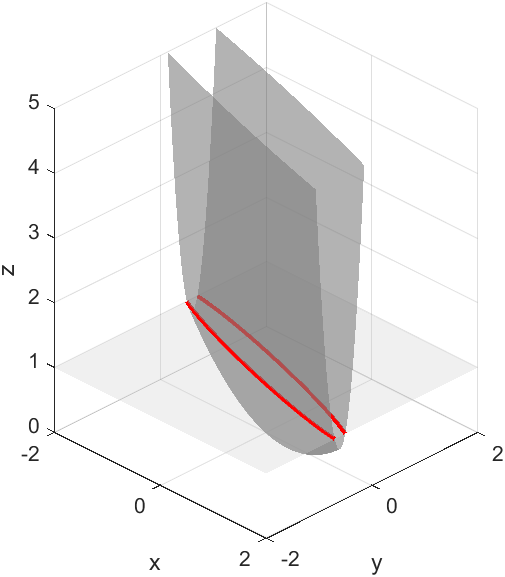
\includegraphics[width=0.6\textwidth]{assets/5.4 Positive definition matrix/Ellipse.png}
  \caption{Ellipse of $f(x, y) = 1$}
\end{figure}

Also you can see the minimum point is the origin.

Till now, we can conclude that positive pivots, sum of squares, graph goes up and a
minimum at the origin all connected together.

Don't forget this is just a $2 \times 2$ example. For a general $n \times n$ matrix,
the conclusion is still true.

If the second derivative matrix is like this:
\[
  \begin{bmatrix}
    f_{xx} & f_{xy} \\
    f_{yx} & f_{yy}
  \end{bmatrix}
\]

Then the condition of a minimum is $f_{xx} > 0$ and $f_{xx}f_{yy} - f_{xy}^2 > 0$.
This is just what you have learned in higher mathematics.

\subsubsection{\textbf{Axis theorem}}

Assume a $3 \times 3$ matrix:
\[
  A = \begin{bmatrix}
    2 & -1 & 0 \\
    -1 & 2 & -1 \\
    0 & -1 & 2
  \end{bmatrix}
\]

We know:
\[
  x^{T}Ax = 2x_1^2 - 2x_1x_2 + 2x_2^2 - 2x_2x_3 + 2x_3^2
\]

Here is the figure of $f(x, y, z) = 1$.
\begin{figure}[H]
  \centering
  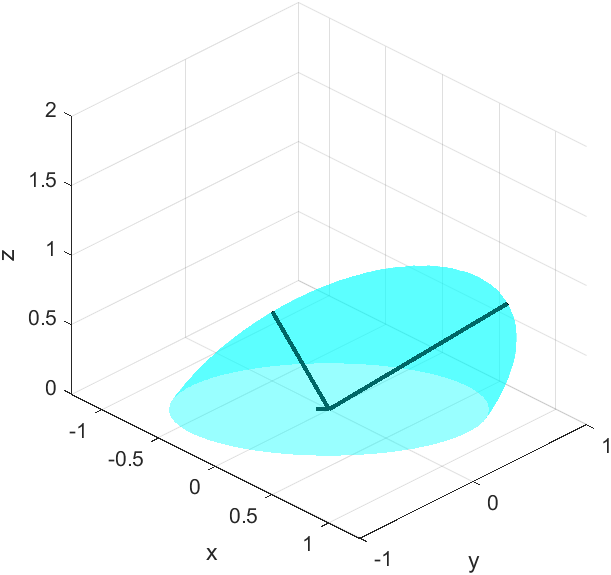
\includegraphics[width=0.6\textwidth]{assets/5.4 Positive definition matrix/Ellipsoid.png}
  \caption{Ellipsoid of $f(x, y, z) = 1$}
\end{figure}

The three axes of the ellipsoid are determined by eigenvectors of $A$ and the lengths
of the axes are determined by eigenvalues of $A$. This is called \textbf{axis theorem}
in physicals, another name of spectral theorem.

\subsection{\textbf{Similar matrix}}

Suppose $A$ and $B$ are \textbf{square} matrices. If there exists a $M$ such that
$B = MAM^{-1}$, then $A$ and $B$ are similar.

The most important property of similar matrices is that they have the same eigenvalues.
\[
  Ax = \lambda x \quad \Rightarrow \quad
  M^{-1}AMM^{-1}x = \lambda M^{-1}x \quad \Rightarrow \quad Bx = \lambda x
\]

But what will happen if there is only 1 eigenvector? Those can be divided into 2
cases. First is $I$, $M^{-1}IM = I$ no matter what $M$ is. The second is called
\textbf{Jordan form}. Before we start, it is necessary to know what is \textbf{Jordan
block}:

\[
  J_i = \begin{bmatrix}
    \lambda & 1 & 0 & \cdots & 0 \\
    0 & \lambda & 1 & \cdots & 0 \\
    0 & 0 & \lambda & \cdots & 0 \\
    \vdots & \vdots & \vdots & \ddots & 1 \\
    0 & 0 & 0 & \cdots & \lambda
  \end{bmatrix}
\]

Jordan form is a block diagonal matrix whose blocks are Jordan blocks. The number of
Jordan blocks is the number of linearly independent eigenvectors.
\[
  J = \begin{bmatrix}
    J_1 & 0 & \cdots & 0 \\
    0 & J_2 & \cdots & 0 \\
    \vdots & \vdots & \ddots & \vdots \\
    0 & 0 & \cdots & J_d
  \end{bmatrix}
\]

And all square matrices are similar to a Jordan form.

When $d = n$, $J = \Lambda$. So diagonalization is a special case of Jordan form. The
other cases are not so good. You have to calculate $J^k$ by hand. Nowadays almost all
ones talk about the good case, diagonalization.

\subsection{\textbf{Singular value decomposition}}

Singular value decomposition (SVD) is the fourth method to factor a matrix. It can be
applied to any $m \times n$ matrix $A$. And it has many applications in data science.

SVD is the best factorization of a matrix. It is more stable than $A = LU$ and more general
than $A = S\Lambda S^{-1}$. It is also the most complicated one:
\[
  A = U\Sigma V^{T}
\]

SVD's idea is to find orthonormal bases of the row space and column space of $A$ and
then map one to another. $U$ and $V$ are orthogonal matrices whose columns are the
orthonormal bases of the column space and row space of $A$. $\Sigma$ is a diagonal
matrix whose diagonal entries are \textbf{singular values} of $A$.

If we multiple both sides by $A^{T}$, then we have:
\[
  A^{T}A = V\Sigma^{T}U^{T}U\Sigma V^{T} = V\Sigma^{T}\Sigma V^{T}
\]

Or:
\[
  A^{T}A = V \begin{bmatrix}
    \sigma_1^2 & 0 & \cdots & 0 \\
    0 & \sigma_2^2 & \cdots & 0 \\
    \vdots & \vdots & \ddots & \vdots \\
    0 & 0 & \cdots & \sigma_n^2
  \end{bmatrix} V^{T}
\]

This is exactly the diagonalization of $A^{T}A$. So the singular values of $A$ are the
square roots of eigenvalues of $A^{T}A$. And $V$ is the matrix whose columns are
eigenvectors of $A^{T}A$. In the same way, we can know that $U$ is the matrix whose columns
are eigenvectors of $AA^{T}$.

The core of SVD is to find the proper basis of the four fundamental subspaces of $A$. Suppose
$r$ is the rank of $A$. Then we have:
\begin{itemize}
  \item $v_1, v_2, \ldots, v_r$ are the orthonormal basis of the row space.
  \item $v_{r+1}, v_{r+2}, \ldots, v_n$ are the orthonormal basis of the null space.
  \item $u_1, u_2, \ldots, u_r$ are the orthonormal basis of the column space.
  \item $u_{r+1}, u_{r+2}, \ldots, u_m$ are the orthonormal basis of the left null space.
\end{itemize}

Because $Av_i = \sigma_i u_i$ and there are no coupled terms. That proves they are the
proper bases.

\newpage
\thispagestyle{empty}
\begin{center}
    \vspace*{96pt}
    \fontsize{60}{60}\customfont{6}\par
    \fontsize{26}{31.2}\section{\textbf{Linear Transformations}}\par % 标题
    \vspace{25pt}
    \begin{center}
      \fontsize{18}{21.6}\customfont\textit{We must know, we will know!}
    \end{center}
    \begin{flushright}
      \fontsize{18}{21.6}\customfont\textit{--- David Hilbert}
    \end{flushright}
    \vfill
\end{center}

\newpage
\subsection{\textbf{Linear transformation}}

Linear transformation $T$ obeys plus and scalar multiplication, and it's often written as:
\[
  T(cu + dv) = cT(u) + dT(v)
\]

Let's firstly take 2 examples of \textbf{NOT} linear transformation:
\begin{itemize}
  \item Shift the plane by $v_0$.
  \item $T(v) = ||v||$
\end{itemize}

Why?
\begin{align*}
  T_1(u + v) &= u + v + v_0 \neq T_1(u) + T_1(v) \\
  T_2(-u) &= ||u|| \neq -||u||
\end{align*}

Operations like rotation and projection are linear transformations. And all linear
transformations can be represented by matrices. That means $T(v) = Av$.

Besides, if you want to know the information of all outputs of $T$, you just need to
know $T(v_1), T(v_2), \ldots, T(v_n)$, namely the basis vectors of the input space.
This is self-proved by the linear property.

And as long as the basis vectors are known, the coordinates of $T(v)$ in the output space
are also known. This is how linear transformations relates to coordinates.

Suppose input space $V$ and output space $W$ both have basis vectors. Then we have:
\[
  AV = W \quad \textbf{or} \quad Av_i = w_i
\]

$v_i$ represents the coordinates of input space, and $w_i$ represents which in output space.

\subsection{\textbf{Change of basis}}
\subsubsection{\textbf{Compression of image}}
Suppose there is a $512 \times 512$ grayscale image $A$. A pixel means an entries of $A$.
Usually a pixel contains 8 bits $x_i$, which means 256 levels of gray. So $x$ is in $R^{512^2}$.
This is a huge space and it's impossible to transport. So we need to compress it.

The main idea is to change the basis. Most of the pixels are similar to their neighbors. So
we can use a new basis to represent the image. The new basis is like:

\[
  v_1 = \begin{bmatrix}
    1 \\ 1 \\ 1 \\ \vdots \\ 1
  \end{bmatrix}, \quad
  v_2 = \begin{bmatrix}
    1 \\ 1 \\ 1 \\ \vdots \\ -1
  \end{bmatrix}, \quad
  v_3 = \begin{bmatrix}
    1 \\ 1 \\ -1 \\ \vdots \\ 0
  \end{bmatrix}, \quad \ldots
\]

It's not the only choice. \textbf{JPEG} uses $8 \times 8$ Fourier basis. And it is talked
about in detail in 7.4.

Now we transform signal $x$ to some coefficients $c$ by changing the basis, the next step
is to compress. The main idea is to set a threshold and set all coefficients smaller than it
to 0. In the other words, we only keep the main components of $x$ and our eyes won't feel
the difference.

The compressed coefficients is $\hat{c}$ which contains many 0s. And we can reconstruct
the image by $\hat{x} = V\hat{c}$. This is the whole process of image compression.

\subsubsection{\textbf{Wavelet basis}}

Wavelet basis is another choice of basis. It is more efficient than Fourier basis in
some cases. Here is an example of Haar wavelet basis:
\[
  w_1 = \begin{bmatrix}
    1 \\ 1 \\ 1 \\ 1
  \end{bmatrix}, \quad
  w_2 = \begin{bmatrix}
    1 \\ 1 \\ -1 \\ -1
  \end{bmatrix}, \quad
  w_3 = \begin{bmatrix}
    1 \\ -1 \\ 0 \\ 0
  \end{bmatrix}, \quad
  w_4 = \begin{bmatrix}
    0 \\ 0 \\ 1 \\ -1
  \end{bmatrix}
\]

Suppose a signal $P$, then we can get its coefficients by $c = W^{-1}P$.

A good basis is fast to calculate $W^{-1}$. If we make $W$ orthonormal by dividing each
basis by its length, then $W^{-1} = W^{T}$.

The second property of a good basis is that it can represent the signal efficiently. That means
most coefficients are small and can be set to 0. Wavelet basis is such a good basis because
the last few basis only care about little parts of the signal.

By the way, \textbf{JPEG2000} uses wavelet basis.

\subsubsection{\textbf{Similarity under change of basis}}

Suppose a linear transformation $T$ has two different matrix representations $A$ and $B$
under two different bases. Then $B$ and $A$ are similar.

It seems easy to understand. But we need to prove it.

Assume the bases are $V$ and $W$. Then we have:
\begin{align*}
  T(V) &= AV \\
  T(W) &= BW
\end{align*}

Because $V$ and $W$ are both bases of the same space, there must be a $M$ such that
\[
  W = MV
\]

Then we have:
\begin{align*}
  W' &= T(W) = T(MV) = M T(V) = MAV \\
  W' &= BW = BMV
\end{align*}

Bring them together:
\[
  B = MAM^{-1}
\]

\subsubsection{\textbf{Eigenvector basis}}

If a basis is formed by eigenvectors, then what the $A$ is?

Obviously:
\[
  T(v_i) = \lambda_i v_i \quad \Rightarrow \quad
  AV = \Lambda V \quad \Rightarrow \quad
  A = \Lambda
\]

So the matrix representation of $T$ under the eigenvector basis is a diagonal matrix.
This is the best basis but too hard to find in practice. So we often choose something cheaper
and close to it like wavelet basis.

\subsection{\textbf{Inverse and pseudoinverse}}
\subsubsection{\textbf{Inverse}}
There are 3 kinds of inverse: two-sided inverse, left inverse and right inverse.

For a full rank matrix, the inverse are two-sided:
\[
  AA^{-1} = I = A^{-1}A
\]

If a matrix is full column ranked, it has left inverse:
\[
  A^{-1}_{left} = (A^{T}A)^{-1}A
\]

We can analogize A's right inverse for full row rank:
\[
  A^{-1}_{right} = A^{T}(AA^{T})^{-1}
\]

\subsubsection{\textbf{Pseudoinverse}}

What's the inverse of $r < n $ and $r < m$ normal matrix $A$? We call it \textbf{pseudoinverse}.

For $x$ in row space, we know $Ax$ is in column space. It is a one-to-one correspondence. And
$Ax$ won't go into null space. If there's another $y$ in row space, then $Ax \neq Ay$.

If we don't think about the null space and left null space, then $A$ is invertible. The inverse
of $A$ is its pseudoinverse $A^{+}$.

How to find $A^{+}$? One way comes from SVD.

Suppose $\Sigma$ obeys $r < n$ and $r < m$:
\[
  \Sigma = \begin{bmatrix}
    \sigma_1 & 0 & \cdots & 0 & 0 \\
    0 & \sigma_2 & \cdots & 0 & 0 \\
    \vdots & \vdots & \ddots & \vdots & \vdots \\
    0 & 0 & \cdots & \sigma_r & 0 \\
    0 & 0 & \cdots & 0 & 0 \\
    \end{bmatrix}_{m \times n}
\]

Then we know:
\[
  \Sigma^{+} = \begin{bmatrix}
    1/\sigma_1 & 0 & \cdots & 0 & 0 \\
    0 & 1/\sigma_2 & \cdots & 0 & 0 \\
    \vdots & \vdots & \ddots & \vdots & \vdots \\
    0 & 0 & \cdots & 1/\sigma_r & 0 \\
    0 & 0 & \cdots & 0 & 0 \\
    \end{bmatrix}_{n \times m}
\]

Also:
\[
  A^{+} = V\Sigma^{+}U^{T}
\]



\newpage
\thispagestyle{empty}
\begin{center}
    \vspace*{96pt}
    \fontsize{60}{60}\customfont{7}\par
    \fontsize{26}{31.2}\section{\textbf{Applications}}\par % 标题
    \vspace{25pt}
    \begin{center}
      \fontsize{18}{21.6}\customfont\textit{Changed and yet the same, I rise again.}
    \end{center}
    \begin{flushright}
      \fontsize{18}{21.6}\customfont\textit{--- Jacob Bernoulli}
    \end{flushright}
    \vfill
\end{center}

\newpage
\subsection{\textbf{Solution of $u_{k+1} = Au_k$}}
\subsubsection{\textbf{Derivation}}

$u_{k+1} = Au_k$ is a typical difference equation. And we can rewrite it to:
\[
  u_k = A^k u_0
\]

Then we can diagonalize $u_k$:
\begin{align*}
  u_0 &= c_1 x_1 + c_2 x_2 + \cdots + c_n x_n = Sc \\
  u_k &= A^k u_0 = S\Lambda^k S^{-1}Sc = S\Lambda^k c
\end{align*}

This is the general solution of $u_{k+1} = Au_k$. And we can see that the eigenvalues
determine the behavior of $u_k$.

\subsubsection{\textbf{Fibonacci sequence}}

Take an example of Fibonacci sequence:
\[
  \begin{bmatrix}
    F_{k+1} \\
    F_k
  \end{bmatrix} =
  \begin{bmatrix}
    1 & 1 \\
    1 & 0
  \end{bmatrix}
  \begin{bmatrix}
    F_k \\
    F_{k-1}
  \end{bmatrix}
\]

We can calculate the eigenvalues and eigenvectors of $A$:
\begin{align*}
  \lambda_1 &= \frac{1 + \sqrt{5}}{2}, \quad
  x_1 = \begin{bmatrix}
    \frac{1 + \sqrt{5}}{2} \\
    1
  \end{bmatrix} \\
  \lambda_2 &= \frac{1 - \sqrt{5}}{2}, \quad
  x_2 = \begin{bmatrix}
    \frac{1 - \sqrt{5}}{2} \\
    1
  \end{bmatrix}
\end{align*}

Now we can consider the initial condition:
\[
  u_0 = \begin{bmatrix}
    F_1 \\
    F_0
  \end{bmatrix} =
  \begin{bmatrix}
    1 \\
    0
  \end{bmatrix} =
  c_1 x_1 + c_2 x_2
  \quad \Rightarrow \quad
  c_1 = \frac{1}{\sqrt{5}}, \quad c_2 = -\frac{1}{\sqrt{5}}
\]

Then we have:
\[
  u_k = \frac{1}{\sqrt{5}} \begin{bmatrix}
    \left(\frac{1 + \sqrt{5}}{2}\right)^{k+1} - \left(\frac{1 - \sqrt{5}}{2}\right)^{k+1} \\
    \left(\frac{1 + \sqrt{5}}{2}\right)^k - \left(\frac{1 - \sqrt{5}}{2}\right)^k
  \end{bmatrix}
\]

That means:
\[
  F_n = \frac{1}{\sqrt{5}} \left[
    \left(\frac{1 + \sqrt{5}}{2}\right)^n -
    \left(\frac{1 - \sqrt{5}}{2}\right)^n
  \right]
\]

\subsection{\textbf{Solution of $\frac{du}{dt} = Au$}}
\subsubsection{\textbf{Example}}

$\frac{du}{dt} = Au$ is a typical differential equation. Let's see an example first:
\begin{align*}
  \frac{du_1}{dt} &= -u_1 + 2u_2 \\
  \frac{du_2}{dt} &= u_1 - 2u_2 \\
  u_0 &= \begin{bmatrix} 1 \\ 0 \end{bmatrix}
\end{align*}

Upon this we can infer that:
\begin{align*}
  A = \begin{bmatrix}
    -1 & 2 \\
    1 & -2
  \end{bmatrix}
  \quad \Rightarrow \quad
  \lambda_1 &= 0, \quad x_1 = \begin{bmatrix} 1 \\ 1/2 \end{bmatrix} \\
  \lambda_2 &= -3, \quad x_2 = \begin{bmatrix} 1 \\ -1 \end{bmatrix}
\end{align*}

The solution is:
\[
  u(t) = c_1 e^{\lambda_1 t} x_1 + c_2 e^{\lambda_2 t} x_2
  = c_1 \begin{bmatrix}
    1 \\
    1/2
  \end{bmatrix} +
  c_2 e^{-3t} \begin{bmatrix}
    1 \\
    -1
  \end{bmatrix}
\]

And we can get $c_1 = c_2 = 1/3$ by the initial condition. So the final solution is:
\[
  u(t) = \frac13 (\begin{bmatrix}
    1 \\
    1/2
  \end{bmatrix} +
  e^{-3t} \begin{bmatrix}
    1 \\
    -1
  \end{bmatrix})
\]

\subsubsection{\textbf{Stability analysis}}

Now jump out the example and consider the stability of $u(t)$. $u(t) \to 0$ no matter what
$u_0$ is when all eigenvalues of $A$ are negative. And there must be point out that if
the complex part is considered, then the condition becomes $Re[\lambda] < 0$.

What about the steady state? This happens when 1 eigenvalue is 0 and all others are
negative. And the steady state is in the direction of the eigenvector whose eigenvalue
is 0. This is the case in the example above.

And if there is an eigenvalue whose real part is positive, then $u(t)$ blows up.

We usually pay the most attention to the stability of second-order systems. In linear
algebra, this means that $A$ is a $2 \times 2$ matrix. And it is stable when $trace(A) < 0$
and $\det A > 0$.

\subsubsection{\textbf{General solution}}

For $\frac{du}{dt} = Au$, $A$ means $u_1$ and $u_2$ are coupled. If we want to
decouple them, we should diagonalize $A$. Set $u = Sv$, then we have:
\[
  \frac{dv}{dt} = S^{-1}ASv = \Lambda v
\]

This leads to:
\[
  \frac{dv_i}{dt} = \lambda_i v_i \quad \Rightarrow \quad v_i = c_i e^{\lambda_i t}
\]

Or:
\[
  v(t) = e^{\Lambda t} v(0) \quad \Rightarrow \quad u(t) = Se^{\Lambda t}S^{-1}u(0)
  = e^{At}u(0)
\]

$e^{At}$ is often called \textbf{matrix exponential}. And it obeys Taylor's expansion:
\[
  e^{At} = I + At + \frac{(At)^2}{2!} + \frac{(At)^3}{3!} + \cdots
\]

Obviously, $e^{At}$ goes to 0 when $Re[\lambda] < 0$.

\subsection{\textbf{Markov matrix}}
\subsubsection{\textbf{Definition and properties}}

Markov matrix $A$ is a matrix that all entries positive and all columns sum to 1. This
kind of matrix is widely used in probability and statistics.

Markov matrix has a special eigenvalue $\lambda_1 = 1$. And all other eigenvalues satisfy
$|\lambda_i| < 1$. Here is the proof:

Suppose a column vector $u = \begin{bmatrix}1 & 1 & \ldots & 1\end{bmatrix}^T$, then we
have:
\[
  Au = \begin{bmatrix}
  \sum_{i=1}^{n} a_{1i} \\
  \sum_{i=1}^{n} a_{2i} \\
  \vdots \\
  \sum_{i=1}^{n} a_{ni}
  \end{bmatrix}
  = u
\]

That means $\lambda_1 = 1$ and $x_1 = u$.

Moreover, Markov matrix represents a probability system that the sum of all states is 1.
So if a probability vector $v$ satisfies $\sum_{i=1}^{n} v_i = 1$, then $Av$ also
satisfies this. If there is an eigenvalue bigger than 1 in absolute value, then $A^k v$
will blow up. This is contradictory. So all other eigenvalues satisfy $|\lambda_i| < 1$.

\subsubsection{\textbf{Usage}}

Markov matrix can be used to solve steady state problems. Suppose $u_{k+1} = Au_k$.

Assume we have been counting the population of two cities $m$ and $n$ for many years.
And we find that every year, 90\% of $m$'s population stays in $m$, and 10\% moves to
$n$. For city $n$, 80\% of its population stays in $n$, and 20\% moves to $m$. Now we
want to know the population distribution of $m$ and $n$ in the long run. Then we have:
\[
  A = \begin{bmatrix}
    0.9 & 0.2 \\
    0.1 & 0.8
  \end{bmatrix}
  \quad \text{and} \quad
  \begin{bmatrix}
    m_{k+1} \\
    n_{k+1}
  \end{bmatrix} =
  A \begin{bmatrix}
    m_k \\
    n_k
  \end{bmatrix}
\]

And we assume the initial population is:
\[
  u_0 = \begin{bmatrix}
    m_0 \\
    n_0
  \end{bmatrix} =
  \begin{bmatrix}
    0 \\
    1000
  \end{bmatrix}
\]

Then we can calculate the eigenvalues and eigenvectors of $A$:
\begin{align*}
  \lambda_1 &= 1, \quad x_1 = \begin{bmatrix} 2 \\ 1 \end{bmatrix} \\
  \lambda_2 &= 0.7, \quad x_2 = \begin{bmatrix} -1 \\ 1 \end{bmatrix}
\end{align*}

And we can get $c_1 = 1000/3, c_2 = 2000/3$ by the initial condition. So the final
solution is:
\[
  u_k = \frac{1000}{3} \begin{bmatrix}
    2 \\
    1
  \end{bmatrix} +
  \frac{2000}{3} (0.7)^k \begin{bmatrix}
    -1 \\
    1
  \end{bmatrix}
\]

\subsection{\textbf{Fourier series}}
\subsubsection{\textbf{Projections with orthonormal basis}}

For any $v$ in $R^n$, we can project it onto an orthonormal basis $q_1, q_2, \ldots, q_n$:
\[
  v = q_1x_1 + q_2x_2 + \cdots + q_nx_n
\]

In matrix form:
\[
  Qx = \begin{bmatrix}
    q_1 & q_2 & \cdots & q_n
  \end{bmatrix}
  \begin{bmatrix}
    x_1 \\
    x_2 \\
    \vdots \\
    x_n
  \end{bmatrix} = v
\]

So we get:
\[
  x = Q^{-1}v = Q^{T}v \quad \text{or} \quad x_i = q_i^{T}v
\]

This is the basis of Fourier series.

\subsubsection{\textbf{Fourier series}}

Here's Fourier series. Suppose we have a function $f(t)$ defined on $[-\pi, \pi]$.
Then we can expand it to:
\[
  f(t) = a_0 + \sum_{n=1}^{\infty} a_n \cos nt + \sum_{n=1}^{\infty} b_n \sin nt
\]

Fourier found that we can replace $v$ with $f(t)$, and replace $q_i$ with
trigonometric functions.

\textbf{P.S.} The orthogonality of trigonometric functions is not so obvious. You can
verify it by integration. By the way, The dot product of two functions $f(t)$ and $g(t)$
is defined as:
\[
  f \cdot g = \int_{-\pi}^{\pi} f(t)g(t) dt
\]

Now we are going to the last part. How to calculate $a_n$ and $b_n$? Take a look at $a_1$,
we do inner product with $\cos t$ on both sides:
\begin{align*}
  \int_{-\pi}^{\pi} f(t) \cos t dt &= a_0 \int_{-\pi}^{\pi} \cos t dt +
  a_1 \int_{-\pi}^{\pi} \cos^2 t dt +
  a_2 \int_{-\pi}^{\pi} \cos 2t \cos t dt + \cdots \\
  &= a_1 \pi
\end{align*}

So it is clear that:
\[
  a_1 = \frac{1}{\pi} \int_{-\pi}^{\pi} f(t) \cos t dt \quad \text{or} \quad
  a_n = \frac{1}{\pi} \int_{-\pi}^{\pi} f(t) \cos nt dt
\]

Also $b_n$ is in the same way.

\subsection{\textbf{Fast Fourier Transform}}
\subsubsection{\textbf{Complex vectors and complex matrices}}

A complex vector $z$ is in $C^n$, its length is defined as:
\[
  ||z|| = \bar{z}^{T} z \quad \text{or} \quad ||z|| = z^{H} z
\]

Inner product of two complex vectors $y$ and $x$ is changed as well, now it is $y^{H} x$.

For a complex symmetric matrix(or Hermitian matrix) $A$, it is defined as $A^{H} = A$.
We have talked about this in 5.3.

For a orthogonal matrix $Q$, it is defined as $Q^{H}Q = I$. And we also changed its name
to unitary matrix.

\subsubsection{\textbf{Fourier matrix}}

Fourier matrix $F_n$ is a complex matrix whose entries are:
\[
  (F_n)_{ij} = \omega^{(i-1)(j-1)} \quad \text{where} \quad
  \omega = e^{-\frac{2\pi i}{n}}
\]

For example:
\[
  F_4 = \frac12 \begin{bmatrix}
    1 & 1 & 1 & 1 \\
    1 & i & -1 & -i \\
    1 & -1 & 1 & -1 \\
    1 & -i & -1 & i
  \end{bmatrix}
\]

It is obvious that $F_4$ is a orthogonal matrix so $F_4^{-1} = F_4^{H}$.

\subsubsection{\textbf{Fast Fourier Transform}}

If we want to calculate $F_{64}$, we have to write down a $64 \times 64$ matrix. This is
too large. So we need Fast Fourier Transform. Be aware that $\omega_{64} = (\omega_{32})^2$,
so there must be some relations between $F_{64}$ and $F_{32}$.

Here is the relation:
\[
  F_{64} = \begin{bmatrix}
    I_{32} & D_{32} \\
    I_{32} & -D_{32}
  \end{bmatrix}
  \begin{bmatrix}
    F_{32} & 0 \\
    0 & F_{32}
  \end{bmatrix}
  P_{64}
\]

$D_{32}$ is a diagonal matrix whose diagonal entries are $1, \omega, \omega^2,
\ldots, \omega^{31}$. $P_{64}$ is a permutation matrix that rearranges the entries of
a vector from $[x_0, x_1, \ldots, x_{63}]^T$ to \\
$[x_0, x_2, \ldots, x_{62}, x_1, x_3, \ldots, x_{63}]^T$.

Then decompose $F_{32}$ in the same way, and repeat this process until $F_1$.

Fast Fourier Transform reduces the complexity of calculating $F_n$ from $O(n^2)$ to
$O(n \log n)$ (Actually $\frac12 n \log n$). If $n = 1024$, then $n^2 = 1048576$ and
$\frac12 n \log n = 5120$. This is a huge improvement. So Fast Fourier Transform is widely
used in almost all fields of science and engineering and greatly changes our world.

\newpage
\section{\textbf{Afterwords}}

Months ago I talked with EE's dean Teacher Chen, he asked me the opinion of
this course. I appreciated it quite a lot. But not everyone agreed with me. Many students
of 2024 cohort said no. Teacher Chen told me EE would not attend Prof.\ Liu's course any more.
I felt bad. That's the origin of this tutorial.

This tutorial is started in the end of August. At that time I was full of hope that I must
finish it before the semester starts and give it to my junior students. But I was too
optimistic. I never thought that Prof.\ Liu quitted. He said he was too busy and wanted to
focus on his Principles of Computer Organization course. It's hard for me to accept this
reality as I said linear algebra was the best course I have ever taken in my college life.

But it had happened. Till then I have written at least 85\% of the tutorial. I have to finish
it with misery. And I know, like every tutorial I wrote, not much students will read it.
It is more like my vanity to show off something. But I think it's worthy, even if only one
reads.

I will continue to finish \textit{Introduction to Compressed Sensing} after this tutorial.
I hope I can finish it before the end of this year. Then I can leave it to Teacher Xue for
her students.

I don't know whether there will be someone to continue my legacy when I graduate. There must
be many mistakes waiting for correction. If you find any, please contact me.

Well, I am really afraid. Not only my graduation, but also my junior students. Maybe all
university are suffering this, students are not willing to learn any more. They just want to
play games and waste time idly. I don't know why or how to change it. Only I can do is to
write tutorials for those who still have a bit ambition. Decades ago we students were
curious and eager, now we are indifferent and lazy. We can't blame society for everything.
Think about ourselves, what a shame!

Hope all I see is just a bad dream. We will be better in the future. Also thank you reading
this far. See you next time!

\begin{flushright}
  Lancet Ross \\
  Sept 3rd, 2025
\end{flushright}

\end{document}